\documentclass[12pt]{article}
\usepackage{fontspec}
\setmainfont{DejaVu Sans}
\usepackage[cm]{fullpage}
\usepackage{graphicx}
\usepackage{tikz}

\begin{document}
\title{CS22310 Hotel Project}
\author{Felix Farquharson}

\maketitle
\tableofcontents

\section{Introduction}
The purpose of this project is to create a prototype hotel booking system
that follows all usability pricipals. Careful attention was to be paid to
the general layouts and navigation parts of the website.

We were to carry a full task analysis, create a full prototype and discuss
general issues and improvements on what we had created at the end of the 
project.

\section{Task Analysis}
\subsection{Needs of System}
There are many reasons to implement a system such as this. Two of the most
significant reasons are: That it will reduce the workload on staff that 
deal with bookings which may lead to lower costs. Also it will improve 
your customer reach by being available 24/7.

An analysis of further needs follows.

\subsection{Who is involved (Target Audience)?}
Obviously there are a number of different parties that will be affected by
the implimentation of a computer based system. The two most obvious will be
hotel staff and potential customers to the business.
\subsubsection{Rich Picture}
A rich picture has been produced to illistrate the different people who will
be affected by the new system.

% Graphic for TeX using PGF
% Title: /home/felix/hotelproject/doc/diagrams/rich_pic.dia
% Creator: Dia v0.97.2
% CreationDate: Sun Apr 14 20:15:31 2013
% For: felix
% \usepackage{tikz}
% The following commands are not supported in PSTricks at present
% We define them conditionally, so when they are implemented,
% this pgf file will use them.
\ifx\du\undefined
  \newlength{\du}
\fi
\setlength{\du}{15\unitlength}
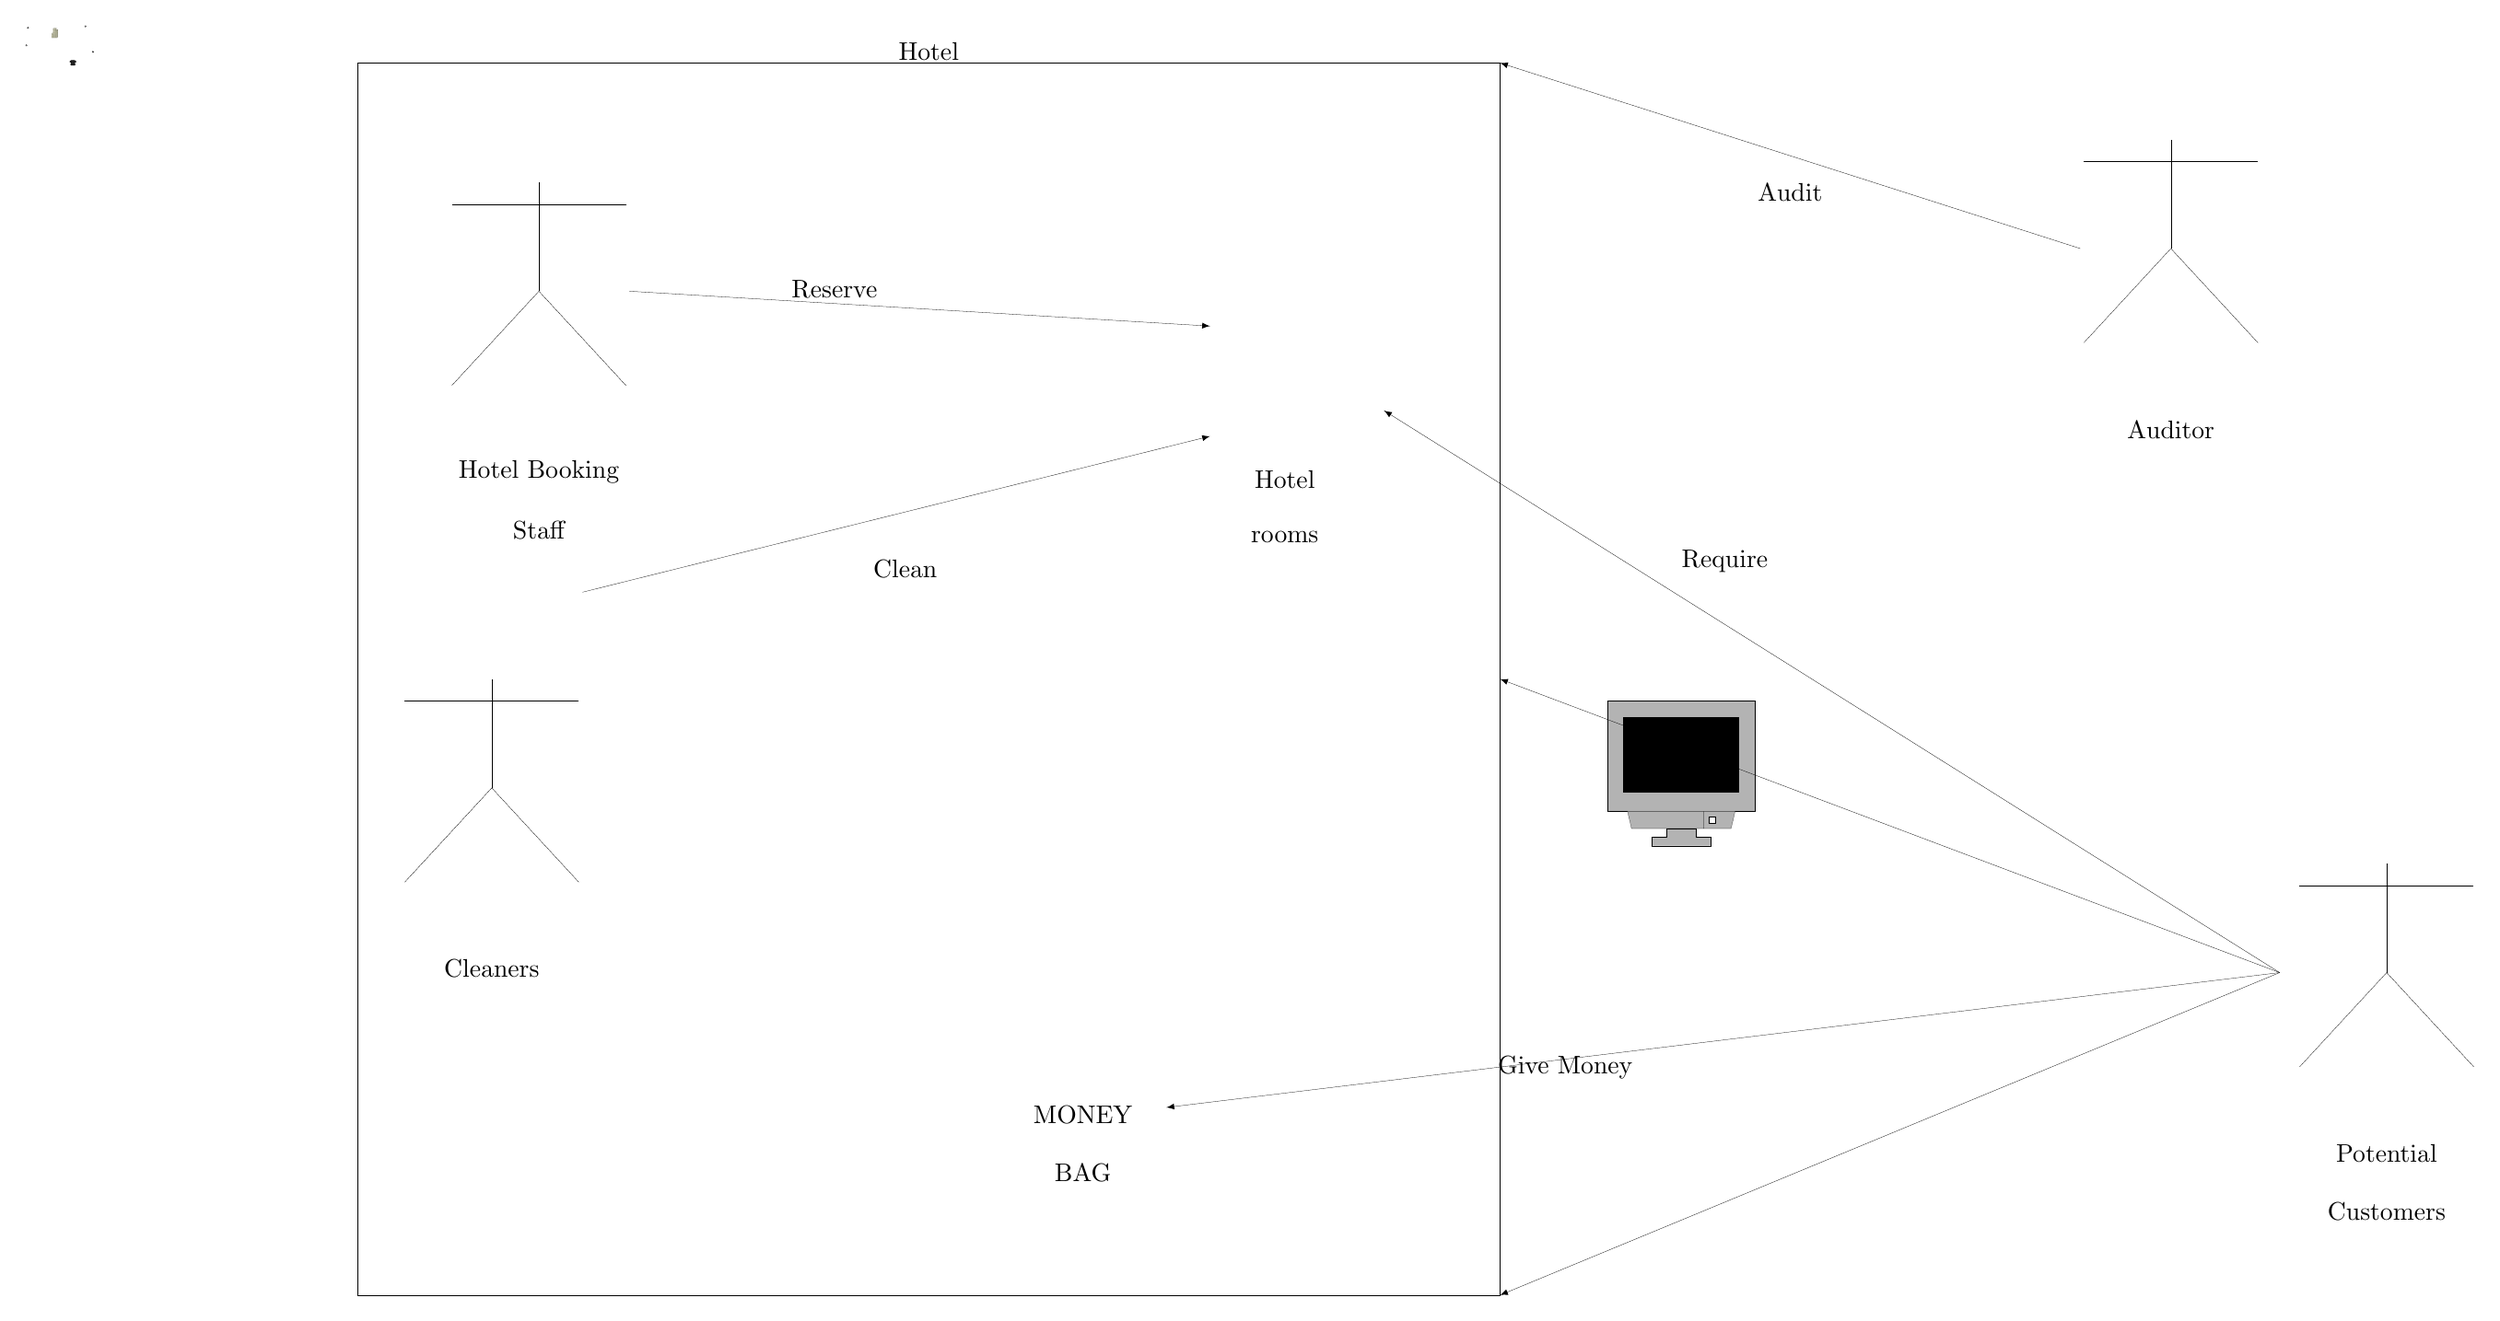
\begin{tikzpicture}
\pgftransformxscale{1.000000}
\pgftransformyscale{-1.000000}
\definecolor{dialinecolor}{rgb}{0.000000, 0.000000, 0.000000}
\pgfsetstrokecolor{dialinecolor}
\definecolor{dialinecolor}{rgb}{1.000000, 1.000000, 1.000000}
\pgfsetfillcolor{dialinecolor}
\pgfsetlinewidth{0.100000\du}
\pgfsetdash{}{0pt}
\pgfsetdash{}{0pt}
\pgfsetmiterjoin
\definecolor{dialinecolor}{rgb}{0.000000, 0.000000, 0.000000}
\pgfsetstrokecolor{dialinecolor}
\draw (4.800000\du,0.550000\du)--(4.800000\du,17.550000\du)--(20.550000\du,17.550000\du)--(20.550000\du,0.550000\du)--cycle;
\pgfsetlinewidth{0.100000\du}
\pgfsetdash{}{0pt}
\definecolor{dialinecolor}{rgb}{1.000000, 1.000000, 1.000000}
\pgfsetfillcolor{dialinecolor}
\pgfpathellipse{\pgfpoint{7.300000\du}{1.900000\du}}{\pgfpoint{0.300000\du}{0\du}}{\pgfpoint{0\du}{0.300000\du}}
\pgfusepath{fill}
\definecolor{dialinecolor}{rgb}{0.000000, 0.000000, 0.000000}
\pgfsetstrokecolor{dialinecolor}
\pgfpathellipse{\pgfpoint{7.300000\du}{1.900000\du}}{\pgfpoint{0.300000\du}{0\du}}{\pgfpoint{0\du}{0.300000\du}}
\pgfusepath{stroke}
\definecolor{dialinecolor}{rgb}{0.000000, 0.000000, 0.000000}
\pgfsetstrokecolor{dialinecolor}
\draw (6.100000\du,2.500000\du)--(8.500000\du,2.500000\du);
\definecolor{dialinecolor}{rgb}{0.000000, 0.000000, 0.000000}
\pgfsetstrokecolor{dialinecolor}
\draw (7.300000\du,2.200000\du)--(7.300000\du,3.700000\du);
\definecolor{dialinecolor}{rgb}{0.000000, 0.000000, 0.000000}
\pgfsetstrokecolor{dialinecolor}
\draw (7.300000\du,3.700000\du)--(6.100000\du,5.000000\du);
\definecolor{dialinecolor}{rgb}{0.000000, 0.000000, 0.000000}
\pgfsetstrokecolor{dialinecolor}
\draw (7.300000\du,3.700000\du)--(8.500000\du,5.000000\du);
% setfont left to latex
\definecolor{dialinecolor}{rgb}{0.000000, 0.000000, 0.000000}
\pgfsetstrokecolor{dialinecolor}
\node at (7.300000\du,6.195000\du){Hotel Booking};
% setfont left to latex
\definecolor{dialinecolor}{rgb}{0.000000, 0.000000, 0.000000}
\pgfsetstrokecolor{dialinecolor}
\node at (7.300000\du,6.995000\du){Staff};
\pgfsetlinewidth{0.100000\du}
\pgfsetdash{}{0pt}
\definecolor{dialinecolor}{rgb}{1.000000, 1.000000, 1.000000}
\pgfsetfillcolor{dialinecolor}
\pgfpathellipse{\pgfpoint{32.775000\du}{11.300000\du}}{\pgfpoint{0.300000\du}{0\du}}{\pgfpoint{0\du}{0.300000\du}}
\pgfusepath{fill}
\definecolor{dialinecolor}{rgb}{0.000000, 0.000000, 0.000000}
\pgfsetstrokecolor{dialinecolor}
\pgfpathellipse{\pgfpoint{32.775000\du}{11.300000\du}}{\pgfpoint{0.300000\du}{0\du}}{\pgfpoint{0\du}{0.300000\du}}
\pgfusepath{stroke}
\definecolor{dialinecolor}{rgb}{0.000000, 0.000000, 0.000000}
\pgfsetstrokecolor{dialinecolor}
\draw (31.575000\du,11.900000\du)--(33.975000\du,11.900000\du);
\definecolor{dialinecolor}{rgb}{0.000000, 0.000000, 0.000000}
\pgfsetstrokecolor{dialinecolor}
\draw (32.775000\du,11.600000\du)--(32.775000\du,13.100000\du);
\definecolor{dialinecolor}{rgb}{0.000000, 0.000000, 0.000000}
\pgfsetstrokecolor{dialinecolor}
\draw (32.775000\du,13.100000\du)--(31.575000\du,14.400000\du);
\definecolor{dialinecolor}{rgb}{0.000000, 0.000000, 0.000000}
\pgfsetstrokecolor{dialinecolor}
\draw (32.775000\du,13.100000\du)--(33.975000\du,14.400000\du);
% setfont left to latex
\definecolor{dialinecolor}{rgb}{0.000000, 0.000000, 0.000000}
\pgfsetstrokecolor{dialinecolor}
\node at (32.775000\du,15.595000\du){Potential};
% setfont left to latex
\definecolor{dialinecolor}{rgb}{0.000000, 0.000000, 0.000000}
\pgfsetstrokecolor{dialinecolor}
\node at (32.775000\du,16.395000\du){Customers};
\pgfsetlinewidth{0.100000\du}
\pgfsetdash{}{0pt}
\pgfsetdash{}{0pt}
\pgfsetbuttcap
\pgfsetmiterjoin
\pgfsetbuttcap
\pgfsetmiterjoin
\pgfsetdash{}{0pt}
\definecolor{dialinecolor}{rgb}{0.133333, 0.133333, 0.133333}
\pgfsetfillcolor{dialinecolor}
\pgfpathmoveto{\pgfpoint{24.900000\du}{14.600000\du}}
\pgfpathcurveto{\pgfpoint{25.090476\du}{14.600000\du}}{\pgfpoint{25.852381\du}{14.695238\du}}{\pgfpoint{26.042857\du}{14.885714\du}}
\pgfpathcurveto{\pgfpoint{26.233333\du}{15.076190\du}}{\pgfpoint{26.233333\du}{15.361905\du}}{\pgfpoint{26.042857\du}{15.457143\du}}
\pgfpathcurveto{\pgfpoint{25.852381\du}{15.552381\du}}{\pgfpoint{25.471429\du}{15.266667\du}}{\pgfpoint{25.471429\du}{15.171429\du}}
\pgfpathcurveto{\pgfpoint{25.471429\du}{15.076190\du}}{\pgfpoint{25.661905\du}{15.076190\du}}{\pgfpoint{25.566667\du}{14.980952\du}}
\pgfpathcurveto{\pgfpoint{25.471429\du}{14.885714\du}}{\pgfpoint{25.471429\du}{14.980952\du}}{\pgfpoint{25.376190\du}{14.980952\du}}
\pgfpathcurveto{\pgfpoint{25.280952\du}{14.980952\du}}{\pgfpoint{25.376190\du}{14.980952\du}}{\pgfpoint{25.376190\du}{15.076190\du}}
\pgfpathcurveto{\pgfpoint{25.376190\du}{15.171429\du}}{\pgfpoint{25.376190\du}{15.361905\du}}{\pgfpoint{25.471429\du}{15.361905\du}}
\pgfpathcurveto{\pgfpoint{25.566667\du}{15.361905\du}}{\pgfpoint{25.566667\du}{15.361905\du}}{\pgfpoint{25.566667\du}{15.457143\du}}
\pgfpathcurveto{\pgfpoint{25.566667\du}{15.552381\du}}{\pgfpoint{25.757143\du}{16.028571\du}}{\pgfpoint{25.757143\du}{16.219048\du}}
\pgfpathcurveto{\pgfpoint{25.757143\du}{16.409524\du}}{\pgfpoint{25.852381\du}{16.600000\du}}{\pgfpoint{25.661905\du}{16.600000\du}}
\pgfpathcurveto{\pgfpoint{25.471429\du}{16.600000\du}}{\pgfpoint{24.328571\du}{16.600000\du}}{\pgfpoint{24.138095\du}{16.600000\du}}
\pgfpathcurveto{\pgfpoint{23.947619\du}{16.600000\du}}{\pgfpoint{24.042857\du}{16.409524\du}}{\pgfpoint{24.042857\du}{16.219048\du}}
\pgfpathcurveto{\pgfpoint{24.042857\du}{16.028571\du}}{\pgfpoint{24.233333\du}{15.552381\du}}{\pgfpoint{24.233333\du}{15.457143\du}}
\pgfpathcurveto{\pgfpoint{24.233333\du}{15.361905\du}}{\pgfpoint{24.233333\du}{15.361905\du}}{\pgfpoint{24.328571\du}{15.361905\du}}
\pgfpathcurveto{\pgfpoint{24.423810\du}{15.361905\du}}{\pgfpoint{24.423810\du}{15.171429\du}}{\pgfpoint{24.423810\du}{15.076190\du}}
\pgfpathcurveto{\pgfpoint{24.423810\du}{14.980952\du}}{\pgfpoint{24.519048\du}{14.980952\du}}{\pgfpoint{24.423810\du}{14.980952\du}}
\pgfpathcurveto{\pgfpoint{24.328571\du}{14.980952\du}}{\pgfpoint{24.328571\du}{14.885714\du}}{\pgfpoint{24.233333\du}{14.980952\du}}
\pgfpathcurveto{\pgfpoint{24.138095\du}{15.076190\du}}{\pgfpoint{24.328571\du}{15.076190\du}}{\pgfpoint{24.328571\du}{15.171429\du}}
\pgfpathcurveto{\pgfpoint{24.328571\du}{15.266667\du}}{\pgfpoint{23.947619\du}{15.552381\du}}{\pgfpoint{23.757143\du}{15.457143\du}}
\pgfpathcurveto{\pgfpoint{23.566667\du}{15.361905\du}}{\pgfpoint{23.566667\du}{15.076190\du}}{\pgfpoint{23.757143\du}{14.885714\du}}
\pgfpathcurveto{\pgfpoint{23.947619\du}{14.695238\du}}{\pgfpoint{24.709524\du}{14.600000\du}}{\pgfpoint{24.900000\du}{14.600000\du}}
\pgfusepath{fill}
\definecolor{dialinecolor}{rgb}{0.000000, 0.000000, 0.000000}
\pgfsetstrokecolor{dialinecolor}
\pgfpathmoveto{\pgfpoint{24.900000\du}{14.600000\du}}
\pgfpathcurveto{\pgfpoint{25.090476\du}{14.600000\du}}{\pgfpoint{25.852381\du}{14.695238\du}}{\pgfpoint{26.042857\du}{14.885714\du}}
\pgfpathcurveto{\pgfpoint{26.233333\du}{15.076190\du}}{\pgfpoint{26.233333\du}{15.361905\du}}{\pgfpoint{26.042857\du}{15.457143\du}}
\pgfpathcurveto{\pgfpoint{25.852381\du}{15.552381\du}}{\pgfpoint{25.471429\du}{15.266667\du}}{\pgfpoint{25.471429\du}{15.171429\du}}
\pgfpathcurveto{\pgfpoint{25.471429\du}{15.076190\du}}{\pgfpoint{25.661905\du}{15.076190\du}}{\pgfpoint{25.566667\du}{14.980952\du}}
\pgfpathcurveto{\pgfpoint{25.471429\du}{14.885714\du}}{\pgfpoint{25.471429\du}{14.980952\du}}{\pgfpoint{25.376190\du}{14.980952\du}}
\pgfpathcurveto{\pgfpoint{25.280952\du}{14.980952\du}}{\pgfpoint{25.376190\du}{14.980952\du}}{\pgfpoint{25.376190\du}{15.076190\du}}
\pgfpathcurveto{\pgfpoint{25.376190\du}{15.171429\du}}{\pgfpoint{25.376190\du}{15.361905\du}}{\pgfpoint{25.471429\du}{15.361905\du}}
\pgfpathcurveto{\pgfpoint{25.566667\du}{15.361905\du}}{\pgfpoint{25.566667\du}{15.361905\du}}{\pgfpoint{25.566667\du}{15.457143\du}}
\pgfpathcurveto{\pgfpoint{25.566667\du}{15.552381\du}}{\pgfpoint{25.757143\du}{16.028571\du}}{\pgfpoint{25.757143\du}{16.219048\du}}
\pgfpathcurveto{\pgfpoint{25.757143\du}{16.409524\du}}{\pgfpoint{25.852381\du}{16.600000\du}}{\pgfpoint{25.661905\du}{16.600000\du}}
\pgfpathcurveto{\pgfpoint{25.471429\du}{16.600000\du}}{\pgfpoint{24.328571\du}{16.600000\du}}{\pgfpoint{24.138095\du}{16.600000\du}}
\pgfpathcurveto{\pgfpoint{23.947619\du}{16.600000\du}}{\pgfpoint{24.042857\du}{16.409524\du}}{\pgfpoint{24.042857\du}{16.219048\du}}
\pgfpathcurveto{\pgfpoint{24.042857\du}{16.028571\du}}{\pgfpoint{24.233333\du}{15.552381\du}}{\pgfpoint{24.233333\du}{15.457143\du}}
\pgfpathcurveto{\pgfpoint{24.233333\du}{15.361905\du}}{\pgfpoint{24.233333\du}{15.361905\du}}{\pgfpoint{24.328571\du}{15.361905\du}}
\pgfpathcurveto{\pgfpoint{24.423810\du}{15.361905\du}}{\pgfpoint{24.423810\du}{15.171429\du}}{\pgfpoint{24.423810\du}{15.076190\du}}
\pgfpathcurveto{\pgfpoint{24.423810\du}{14.980952\du}}{\pgfpoint{24.519048\du}{14.980952\du}}{\pgfpoint{24.423810\du}{14.980952\du}}
\pgfpathcurveto{\pgfpoint{24.328571\du}{14.980952\du}}{\pgfpoint{24.328571\du}{14.885714\du}}{\pgfpoint{24.233333\du}{14.980952\du}}
\pgfpathcurveto{\pgfpoint{24.138095\du}{15.076190\du}}{\pgfpoint{24.328571\du}{15.076190\du}}{\pgfpoint{24.328571\du}{15.171429\du}}
\pgfpathcurveto{\pgfpoint{24.328571\du}{15.266667\du}}{\pgfpoint{23.947619\du}{15.552381\du}}{\pgfpoint{23.757143\du}{15.457143\du}}
\pgfpathcurveto{\pgfpoint{23.566667\du}{15.361905\du}}{\pgfpoint{23.566667\du}{15.076190\du}}{\pgfpoint{23.757143\du}{14.885714\du}}
\pgfpathcurveto{\pgfpoint{23.947619\du}{14.695238\du}}{\pgfpoint{24.709524\du}{14.600000\du}}{\pgfpoint{24.900000\du}{14.600000\du}}
\pgfusepath{stroke}
\pgfsetbuttcap
\pgfsetmiterjoin
\pgfsetdash{}{0pt}
\definecolor{dialinecolor}{rgb}{0.466667, 0.466667, 0.466667}
\pgfsetfillcolor{dialinecolor}
\pgfpathellipse{\pgfpoint{24.900000\du}{15.476190\du}}{\pgfpoint{0.400000\du}{0\du}}{\pgfpoint{0\du}{0.400000\du}}
\pgfusepath{fill}
\definecolor{dialinecolor}{rgb}{0.000000, 0.000000, 0.000000}
\pgfsetstrokecolor{dialinecolor}
\pgfpathellipse{\pgfpoint{24.900000\du}{15.476190\du}}{\pgfpoint{0.400000\du}{0\du}}{\pgfpoint{0\du}{0.400000\du}}
\pgfusepath{stroke}
\pgfsetbuttcap
\pgfsetmiterjoin
\pgfsetdash{}{0pt}
\definecolor{dialinecolor}{rgb}{0.800000, 0.800000, 0.800000}
\pgfsetfillcolor{dialinecolor}
\pgfpathellipse{\pgfpoint{25.109524\du}{15.266667\du}}{\pgfpoint{0.057143\du}{0\du}}{\pgfpoint{0\du}{0.057143\du}}
\pgfusepath{fill}
\definecolor{dialinecolor}{rgb}{0.000000, 0.000000, 0.000000}
\pgfsetstrokecolor{dialinecolor}
\pgfpathellipse{\pgfpoint{25.109524\du}{15.266667\du}}{\pgfpoint{0.057143\du}{0\du}}{\pgfpoint{0\du}{0.057143\du}}
\pgfusepath{stroke}
\pgfsetbuttcap
\pgfsetmiterjoin
\pgfsetdash{}{0pt}
\definecolor{dialinecolor}{rgb}{0.800000, 0.800000, 0.800000}
\pgfsetfillcolor{dialinecolor}
\pgfpathellipse{\pgfpoint{24.976190\du}{15.190476\du}}{\pgfpoint{0.057143\du}{0\du}}{\pgfpoint{0\du}{0.057143\du}}
\pgfusepath{fill}
\definecolor{dialinecolor}{rgb}{0.000000, 0.000000, 0.000000}
\pgfsetstrokecolor{dialinecolor}
\pgfpathellipse{\pgfpoint{24.976190\du}{15.190476\du}}{\pgfpoint{0.057143\du}{0\du}}{\pgfpoint{0\du}{0.057143\du}}
\pgfusepath{stroke}
\pgfsetbuttcap
\pgfsetmiterjoin
\pgfsetdash{}{0pt}
\definecolor{dialinecolor}{rgb}{0.800000, 0.800000, 0.800000}
\pgfsetfillcolor{dialinecolor}
\pgfpathellipse{\pgfpoint{24.823810\du}{15.190476\du}}{\pgfpoint{0.057143\du}{0\du}}{\pgfpoint{0\du}{0.057143\du}}
\pgfusepath{fill}
\definecolor{dialinecolor}{rgb}{0.000000, 0.000000, 0.000000}
\pgfsetstrokecolor{dialinecolor}
\pgfpathellipse{\pgfpoint{24.823810\du}{15.190476\du}}{\pgfpoint{0.057143\du}{0\du}}{\pgfpoint{0\du}{0.057143\du}}
\pgfusepath{stroke}
\pgfsetbuttcap
\pgfsetmiterjoin
\pgfsetdash{}{0pt}
\definecolor{dialinecolor}{rgb}{0.800000, 0.800000, 0.800000}
\pgfsetfillcolor{dialinecolor}
\pgfpathellipse{\pgfpoint{24.690476\du}{15.266667\du}}{\pgfpoint{0.057143\du}{0\du}}{\pgfpoint{0\du}{0.057143\du}}
\pgfusepath{fill}
\definecolor{dialinecolor}{rgb}{0.000000, 0.000000, 0.000000}
\pgfsetstrokecolor{dialinecolor}
\pgfpathellipse{\pgfpoint{24.690476\du}{15.266667\du}}{\pgfpoint{0.057143\du}{0\du}}{\pgfpoint{0\du}{0.057143\du}}
\pgfusepath{stroke}
\pgfsetbuttcap
\pgfsetmiterjoin
\pgfsetdash{}{0pt}
\definecolor{dialinecolor}{rgb}{0.800000, 0.800000, 0.800000}
\pgfsetfillcolor{dialinecolor}
\pgfpathellipse{\pgfpoint{24.614286\du}{15.400000\du}}{\pgfpoint{0.057143\du}{0\du}}{\pgfpoint{0\du}{0.057143\du}}
\pgfusepath{fill}
\definecolor{dialinecolor}{rgb}{0.000000, 0.000000, 0.000000}
\pgfsetstrokecolor{dialinecolor}
\pgfpathellipse{\pgfpoint{24.614286\du}{15.400000\du}}{\pgfpoint{0.057143\du}{0\du}}{\pgfpoint{0\du}{0.057143\du}}
\pgfusepath{stroke}
\pgfsetbuttcap
\pgfsetmiterjoin
\pgfsetdash{}{0pt}
\definecolor{dialinecolor}{rgb}{0.800000, 0.800000, 0.800000}
\pgfsetfillcolor{dialinecolor}
\pgfpathellipse{\pgfpoint{24.614286\du}{15.552381\du}}{\pgfpoint{0.057143\du}{0\du}}{\pgfpoint{0\du}{0.057143\du}}
\pgfusepath{fill}
\definecolor{dialinecolor}{rgb}{0.000000, 0.000000, 0.000000}
\pgfsetstrokecolor{dialinecolor}
\pgfpathellipse{\pgfpoint{24.614286\du}{15.552381\du}}{\pgfpoint{0.057143\du}{0\du}}{\pgfpoint{0\du}{0.057143\du}}
\pgfusepath{stroke}
\pgfsetbuttcap
\pgfsetmiterjoin
\pgfsetdash{}{0pt}
\definecolor{dialinecolor}{rgb}{0.800000, 0.800000, 0.800000}
\pgfsetfillcolor{dialinecolor}
\pgfpathellipse{\pgfpoint{24.690476\du}{15.685714\du}}{\pgfpoint{0.057143\du}{0\du}}{\pgfpoint{0\du}{0.057143\du}}
\pgfusepath{fill}
\definecolor{dialinecolor}{rgb}{0.000000, 0.000000, 0.000000}
\pgfsetstrokecolor{dialinecolor}
\pgfpathellipse{\pgfpoint{24.690476\du}{15.685714\du}}{\pgfpoint{0.057143\du}{0\du}}{\pgfpoint{0\du}{0.057143\du}}
\pgfusepath{stroke}
\pgfsetbuttcap
\pgfsetmiterjoin
\pgfsetdash{}{0pt}
\definecolor{dialinecolor}{rgb}{0.800000, 0.800000, 0.800000}
\pgfsetfillcolor{dialinecolor}
\pgfpathellipse{\pgfpoint{24.823810\du}{15.761905\du}}{\pgfpoint{0.057143\du}{0\du}}{\pgfpoint{0\du}{0.057143\du}}
\pgfusepath{fill}
\definecolor{dialinecolor}{rgb}{0.000000, 0.000000, 0.000000}
\pgfsetstrokecolor{dialinecolor}
\pgfpathellipse{\pgfpoint{24.823810\du}{15.761905\du}}{\pgfpoint{0.057143\du}{0\du}}{\pgfpoint{0\du}{0.057143\du}}
\pgfusepath{stroke}
\pgfsetbuttcap
\pgfsetmiterjoin
\pgfsetdash{}{0pt}
\definecolor{dialinecolor}{rgb}{0.800000, 0.800000, 0.800000}
\pgfsetfillcolor{dialinecolor}
\pgfpathellipse{\pgfpoint{24.976190\du}{15.761905\du}}{\pgfpoint{0.057143\du}{0\du}}{\pgfpoint{0\du}{0.057143\du}}
\pgfusepath{fill}
\definecolor{dialinecolor}{rgb}{0.000000, 0.000000, 0.000000}
\pgfsetstrokecolor{dialinecolor}
\pgfpathellipse{\pgfpoint{24.976190\du}{15.761905\du}}{\pgfpoint{0.057143\du}{0\du}}{\pgfpoint{0\du}{0.057143\du}}
\pgfusepath{stroke}
\pgfsetbuttcap
\pgfsetmiterjoin
\pgfsetdash{}{0pt}
\definecolor{dialinecolor}{rgb}{0.800000, 0.800000, 0.800000}
\pgfsetfillcolor{dialinecolor}
\pgfpathellipse{\pgfpoint{25.109524\du}{15.685714\du}}{\pgfpoint{0.057143\du}{0\du}}{\pgfpoint{0\du}{0.057143\du}}
\pgfusepath{fill}
\definecolor{dialinecolor}{rgb}{0.000000, 0.000000, 0.000000}
\pgfsetstrokecolor{dialinecolor}
\pgfpathellipse{\pgfpoint{25.109524\du}{15.685714\du}}{\pgfpoint{0.057143\du}{0\du}}{\pgfpoint{0\du}{0.057143\du}}
\pgfusepath{stroke}
\pgfsetbuttcap
\pgfsetmiterjoin
\pgfsetdash{}{0pt}
\definecolor{dialinecolor}{rgb}{0.666667, 0.666667, 0.666667}
\pgfsetfillcolor{dialinecolor}
\pgfpathellipse{\pgfpoint{24.900000\du}{15.476190\du}}{\pgfpoint{0.190476\du}{0\du}}{\pgfpoint{0\du}{0.190476\du}}
\pgfusepath{fill}
\definecolor{dialinecolor}{rgb}{0.000000, 0.000000, 0.000000}
\pgfsetstrokecolor{dialinecolor}
\pgfpathellipse{\pgfpoint{24.900000\du}{15.476190\du}}{\pgfpoint{0.190476\du}{0\du}}{\pgfpoint{0\du}{0.190476\du}}
\pgfusepath{stroke}
\pgfsetbuttcap
\pgfsetmiterjoin
\pgfsetdash{}{0pt}
\definecolor{dialinecolor}{rgb}{0.666667, 0.666667, 0.666667}
\pgfsetfillcolor{dialinecolor}
\pgfpathmoveto{\pgfpoint{25.185714\du}{15.571429\du}}
\pgfpathcurveto{\pgfpoint{25.223810\du}{15.590476\du}}{\pgfpoint{25.242857\du}{15.571429\du}}{\pgfpoint{25.300000\du}{15.571429\du}}
\pgfpathcurveto{\pgfpoint{25.357143\du}{15.571429\du}}{\pgfpoint{25.338095\du}{15.552381\du}}{\pgfpoint{25.338095\du}{15.590476\du}}
\pgfpathcurveto{\pgfpoint{25.319048\du}{15.628571\du}}{\pgfpoint{25.338095\du}{15.628571\du}}{\pgfpoint{25.280952\du}{15.628571\du}}
\pgfpathcurveto{\pgfpoint{25.223810\du}{15.628571\du}}{\pgfpoint{25.223810\du}{15.647619\du}}{\pgfpoint{25.147619\du}{15.590476\du}}
\pgfpathcurveto{\pgfpoint{25.071429\du}{15.552381\du}}{\pgfpoint{25.128571\du}{15.533333\du}}{\pgfpoint{25.185714\du}{15.571429\du}}
\pgfusepath{fill}
\definecolor{dialinecolor}{rgb}{0.000000, 0.000000, 0.000000}
\pgfsetstrokecolor{dialinecolor}
\pgfpathmoveto{\pgfpoint{25.185714\du}{15.571429\du}}
\pgfpathcurveto{\pgfpoint{25.223810\du}{15.590476\du}}{\pgfpoint{25.242857\du}{15.571429\du}}{\pgfpoint{25.300000\du}{15.571429\du}}
\pgfpathcurveto{\pgfpoint{25.357143\du}{15.571429\du}}{\pgfpoint{25.338095\du}{15.552381\du}}{\pgfpoint{25.338095\du}{15.590476\du}}
\pgfpathcurveto{\pgfpoint{25.319048\du}{15.628571\du}}{\pgfpoint{25.338095\du}{15.628571\du}}{\pgfpoint{25.280952\du}{15.628571\du}}
\pgfpathcurveto{\pgfpoint{25.223810\du}{15.628571\du}}{\pgfpoint{25.223810\du}{15.647619\du}}{\pgfpoint{25.147619\du}{15.590476\du}}
\pgfpathcurveto{\pgfpoint{25.071429\du}{15.552381\du}}{\pgfpoint{25.128571\du}{15.533333\du}}{\pgfpoint{25.185714\du}{15.571429\du}}
\pgfusepath{stroke}
\pgfsetlinewidth{0.100000\du}
\pgfsetdash{}{0pt}
\pgfsetdash{}{0pt}
\pgfsetbuttcap
\pgfsetmiterjoin
\pgfsetlinewidth{0.050000\du}
\pgfsetbuttcap
\pgfsetmiterjoin
\pgfsetdash{}{0pt}
\definecolor{dialinecolor}{rgb}{0.701961, 0.701961, 0.701961}
\pgfsetfillcolor{dialinecolor}
\fill (22.033051\du,9.350000\du)--(22.033051\du,10.875424\du)--(24.066949\du,10.875424\du)--(24.066949\du,9.350000\du)--cycle;
\definecolor{dialinecolor}{rgb}{0.000000, 0.000000, 0.000000}
\pgfsetstrokecolor{dialinecolor}
\draw (22.033051\du,9.350000\du)--(22.033051\du,10.875424\du)--(24.066949\du,10.875424\du)--(24.066949\du,9.350000\du)--cycle;
\pgfsetlinewidth{0.100000\du}
\pgfsetbuttcap
\pgfsetmiterjoin
\pgfsetdash{}{0pt}
\definecolor{dialinecolor}{rgb}{0.000000, 0.000000, 0.000000}
\pgfsetfillcolor{dialinecolor}
\fill (22.253390\du,9.570339\du)--(22.253390\du,10.621186\du)--(23.846610\du,10.621186\du)--(23.846610\du,9.570339\du)--cycle;
\pgfsetlinewidth{0.050000\du}
\pgfsetbuttcap
\pgfsetmiterjoin
\pgfsetdash{}{0pt}
\definecolor{dialinecolor}{rgb}{0.701961, 0.701961, 0.701961}
\pgfsetfillcolor{dialinecolor}
\fill (22.308475\du,10.875424\du)--(23.355085\du,10.875424\du)--(23.355085\du,11.112712\du)--(22.363559\du,11.112712\du)--cycle;
\definecolor{dialinecolor}{rgb}{0.000000, 0.000000, 0.000000}
\pgfsetstrokecolor{dialinecolor}
\draw (22.308475\du,10.875424\du)--(23.355085\du,10.875424\du)--(23.355085\du,11.112712\du)--(22.363559\du,11.112712\du)--cycle;
\pgfsetbuttcap
\pgfsetmiterjoin
\pgfsetdash{}{0pt}
\definecolor{dialinecolor}{rgb}{0.701961, 0.701961, 0.701961}
\pgfsetfillcolor{dialinecolor}
\fill (23.355085\du,10.875424\du)--(23.791525\du,10.875424\du)--(23.736441\du,11.112712\du)--(23.355085\du,11.112712\du)--cycle;
\definecolor{dialinecolor}{rgb}{0.000000, 0.000000, 0.000000}
\pgfsetstrokecolor{dialinecolor}
\draw (23.355085\du,10.875424\du)--(23.791525\du,10.875424\du)--(23.736441\du,11.112712\du)--(23.355085\du,11.112712\du)--cycle;
\pgfsetlinewidth{0.025000\du}
\pgfsetbuttcap
\pgfsetmiterjoin
\pgfsetdash{}{0pt}
\definecolor{dialinecolor}{rgb}{1.000000, 1.000000, 1.000000}
\pgfsetfillcolor{dialinecolor}
\fill (23.426271\du,10.946610\du)--(23.426271\du,11.041525\du)--(23.521186\du,11.041525\du)--(23.521186\du,10.946610\du)--cycle;
\definecolor{dialinecolor}{rgb}{0.000000, 0.000000, 0.000000}
\pgfsetstrokecolor{dialinecolor}
\draw (23.426271\du,10.946610\du)--(23.426271\du,11.041525\du)--(23.521186\du,11.041525\du)--(23.521186\du,10.946610\du)--cycle;
\pgfsetlinewidth{0.050000\du}
\pgfsetbuttcap
\pgfsetmiterjoin
\pgfsetdash{}{0pt}
\definecolor{dialinecolor}{rgb}{0.701961, 0.701961, 0.701961}
\pgfsetfillcolor{dialinecolor}
\fill (22.846610\du,11.112712\du)--(23.253390\du,11.112712\du)--(23.253390\du,11.231356\du)--(23.456780\du,11.231356\du)--(23.456780\du,11.350000\du)--(22.643220\du,11.350000\du)--(22.643220\du,11.231356\du)--(22.846610\du,11.231356\du)--cycle;
\definecolor{dialinecolor}{rgb}{0.000000, 0.000000, 0.000000}
\pgfsetstrokecolor{dialinecolor}
\draw (22.846610\du,11.112712\du)--(23.253390\du,11.112712\du)--(23.253390\du,11.231356\du)--(23.456780\du,11.231356\du)--(23.456780\du,11.350000\du)--(22.643220\du,11.350000\du)--(22.643220\du,11.231356\du)--(22.846610\du,11.231356\du)--cycle;
% setfont left to latex
\definecolor{dialinecolor}{rgb}{0.000000, 0.000000, 0.000000}
\pgfsetstrokecolor{dialinecolor}
\node at (23.050000\du,12.017797\du){};
\pgfsetlinewidth{0.100000\du}
\pgfsetdash{}{0pt}
\pgfsetdash{}{0pt}
\pgfsetbuttcap
\pgfsetmiterjoin
\pgfsetlinewidth{0.001000\du}
\pgfsetbuttcap
\pgfsetmiterjoin
\pgfsetdash{}{0pt}
\definecolor{dialinecolor}{rgb}{0.788235, 0.788235, 0.713726}
\pgfsetfillcolor{dialinecolor}
\pgfpathmoveto{\pgfpoint{16.891855\du}{3.842254\du}}
\pgfpathlineto{\pgfpoint{16.553742\du}{4.181201\du}}
\pgfpathlineto{\pgfpoint{17.068207\du}{4.181201\du}}
\pgfpathlineto{\pgfpoint{17.405903\du}{3.842254\du}}
\pgfpathlineto{\pgfpoint{16.891855\du}{3.842254\du}}
\pgfusepath{fill}
\pgfsetbuttcap
\pgfsetmiterjoin
\pgfsetdash{}{0pt}
\definecolor{dialinecolor}{rgb}{0.286275, 0.286275, 0.211765}
\pgfsetstrokecolor{dialinecolor}
\pgfpathmoveto{\pgfpoint{16.891855\du}{3.842254\du}}
\pgfpathlineto{\pgfpoint{16.553742\du}{4.181201\du}}
\pgfpathlineto{\pgfpoint{17.068207\du}{4.181201\du}}
\pgfpathlineto{\pgfpoint{17.405903\du}{3.842254\du}}
\pgfpathlineto{\pgfpoint{16.891855\du}{3.842254\du}}
\pgfusepath{stroke}
\pgfsetbuttcap
\pgfsetmiterjoin
\pgfsetdash{}{0pt}
\definecolor{dialinecolor}{rgb}{0.478431, 0.478431, 0.352941}
\pgfsetfillcolor{dialinecolor}
\pgfpathmoveto{\pgfpoint{18.082964\du}{2.372650\du}}
\pgfpathlineto{\pgfpoint{18.419826\du}{2.032869\du}}
\pgfpathlineto{\pgfpoint{18.419826\du}{4.779465\du}}
\pgfpathlineto{\pgfpoint{18.082964\du}{5.150514\du}}
\pgfpathlineto{\pgfpoint{18.082964\du}{2.372650\du}}
\pgfusepath{fill}
\pgfsetbuttcap
\pgfsetmiterjoin
\pgfsetdash{}{0pt}
\definecolor{dialinecolor}{rgb}{0.286275, 0.286275, 0.211765}
\pgfsetstrokecolor{dialinecolor}
\pgfpathmoveto{\pgfpoint{18.082964\du}{2.372650\du}}
\pgfpathlineto{\pgfpoint{18.419826\du}{2.032869\du}}
\pgfpathlineto{\pgfpoint{18.419826\du}{4.779465\du}}
\pgfpathlineto{\pgfpoint{18.082964\du}{5.150514\du}}
\pgfpathlineto{\pgfpoint{18.082964\du}{2.372650\du}}
\pgfusepath{stroke}
\pgfsetbuttcap
\pgfsetmiterjoin
\pgfsetdash{}{0pt}
\definecolor{dialinecolor}{rgb}{0.788235, 0.788235, 0.713726}
\pgfsetfillcolor{dialinecolor}
\pgfpathmoveto{\pgfpoint{18.403983\du}{2.566096\du}}
\pgfpathlineto{\pgfpoint{18.082964\du}{2.905876\du}}
\pgfpathlineto{\pgfpoint{18.613272\du}{2.905876\du}}
\pgfpathlineto{\pgfpoint{18.935125\du}{2.566096\du}}
\pgfpathlineto{\pgfpoint{18.403983\du}{2.566096\du}}
\pgfusepath{fill}
\pgfsetbuttcap
\pgfsetmiterjoin
\pgfsetdash{}{0pt}
\definecolor{dialinecolor}{rgb}{0.286275, 0.286275, 0.211765}
\pgfsetstrokecolor{dialinecolor}
\pgfpathmoveto{\pgfpoint{18.403983\du}{2.566096\du}}
\pgfpathlineto{\pgfpoint{18.082964\du}{2.905876\du}}
\pgfpathlineto{\pgfpoint{18.613272\du}{2.905876\du}}
\pgfpathlineto{\pgfpoint{18.935125\du}{2.566096\du}}
\pgfpathlineto{\pgfpoint{18.403983\du}{2.566096\du}}
\pgfusepath{stroke}
\pgfsetbuttcap
\pgfsetmiterjoin
\pgfsetdash{}{0pt}
\definecolor{dialinecolor}{rgb}{0.478431, 0.478431, 0.352941}
\pgfsetfillcolor{dialinecolor}
\pgfpathmoveto{\pgfpoint{18.613272\du}{2.905876\du}}
\pgfpathlineto{\pgfpoint{18.950968\du}{2.566096\du}}
\pgfpathlineto{\pgfpoint{18.950968\du}{5.344377\du}}
\pgfpathlineto{\pgfpoint{18.613272\du}{5.700000\du}}
\pgfpathlineto{\pgfpoint{18.613272\du}{2.905876\du}}
\pgfusepath{fill}
\pgfsetbuttcap
\pgfsetmiterjoin
\pgfsetdash{}{0pt}
\definecolor{dialinecolor}{rgb}{0.286275, 0.286275, 0.211765}
\pgfsetstrokecolor{dialinecolor}
\pgfpathmoveto{\pgfpoint{18.613272\du}{2.905876\du}}
\pgfpathlineto{\pgfpoint{18.949300\du}{2.568180\du}}
\pgfusepath{stroke}
\pgfsetbuttcap
\pgfsetmiterjoin
\pgfsetdash{}{0pt}
\definecolor{dialinecolor}{rgb}{0.286275, 0.286275, 0.211765}
\pgfsetstrokecolor{dialinecolor}
\pgfpathmoveto{\pgfpoint{18.949300\du}{5.346044\du}}
\pgfpathlineto{\pgfpoint{18.613272\du}{5.700000\du}}
\pgfpathlineto{\pgfpoint{18.613272\du}{2.905876\du}}
\pgfusepath{stroke}
\pgfsetbuttcap
\pgfsetmiterjoin
\pgfsetdash{}{0pt}
\definecolor{dialinecolor}{rgb}{0.788235, 0.788235, 0.713726}
\pgfsetfillcolor{dialinecolor}
\pgfpathmoveto{\pgfpoint{17.422580\du}{2.017443\du}}
\pgfpathlineto{\pgfpoint{17.084884\du}{2.356390\du}}
\pgfpathlineto{\pgfpoint{17.084884\du}{2.356390\du}}
\pgfpathlineto{\pgfpoint{18.082964\du}{2.356390\du}}
\pgfpathlineto{\pgfpoint{18.419826\du}{2.017443\du}}
\pgfpathlineto{\pgfpoint{17.422580\du}{2.017443\du}}
\pgfpathlineto{\pgfpoint{17.422580\du}{2.017443\du}}
\pgfusepath{fill}
\pgfsetbuttcap
\pgfsetmiterjoin
\pgfsetdash{}{0pt}
\definecolor{dialinecolor}{rgb}{0.788235, 0.788235, 0.713726}
\pgfsetfillcolor{dialinecolor}
\pgfpathmoveto{\pgfpoint{17.422580\du}{2.017443\du}}
\pgfpathlineto{\pgfpoint{17.084884\du}{2.356390\du}}
\pgfpathlineto{\pgfpoint{18.082964\du}{2.356390\du}}
\pgfpathlineto{\pgfpoint{18.419826\du}{2.017443\du}}
\pgfpathlineto{\pgfpoint{17.422580\du}{2.017443\du}}
\pgfusepath{fill}
\pgfsetbuttcap
\pgfsetmiterjoin
\pgfsetdash{}{0pt}
\definecolor{dialinecolor}{rgb}{0.286275, 0.286275, 0.211765}
\pgfsetstrokecolor{dialinecolor}
\pgfpathmoveto{\pgfpoint{17.422580\du}{2.017443\du}}
\pgfpathlineto{\pgfpoint{17.084884\du}{2.356390\du}}
\pgfpathlineto{\pgfpoint{18.082964\du}{2.356390\du}}
\pgfpathlineto{\pgfpoint{18.419826\du}{2.017443\du}}
\pgfpathlineto{\pgfpoint{17.422580\du}{2.017443\du}}
\pgfusepath{stroke}
\pgfsetbuttcap
\pgfsetmiterjoin
\pgfsetdash{}{0pt}
\definecolor{dialinecolor}{rgb}{0.717647, 0.717647, 0.615686}
\pgfsetfillcolor{dialinecolor}
\pgfpathmoveto{\pgfpoint{16.553742\du}{5.700000\du}}
\pgfpathlineto{\pgfpoint{16.553742\du}{4.181201\du}}
\pgfpathlineto{\pgfpoint{17.084884\du}{4.181201\du}}
\pgfpathlineto{\pgfpoint{17.084884\du}{2.356390\du}}
\pgfpathlineto{\pgfpoint{18.082964\du}{2.356390\du}}
\pgfpathlineto{\pgfpoint{18.082964\du}{2.905876\du}}
\pgfpathlineto{\pgfpoint{18.613272\du}{2.905876\du}}
\pgfpathlineto{\pgfpoint{18.613272\du}{5.700000\du}}
\pgfpathlineto{\pgfpoint{16.553742\du}{5.700000\du}}
\pgfusepath{fill}
\pgfsetbuttcap
\pgfsetmiterjoin
\pgfsetdash{}{0pt}
\definecolor{dialinecolor}{rgb}{0.286275, 0.286275, 0.211765}
\pgfsetstrokecolor{dialinecolor}
\pgfpathmoveto{\pgfpoint{16.553742\du}{5.700000\du}}
\pgfpathlineto{\pgfpoint{16.553742\du}{4.181201\du}}
\pgfpathlineto{\pgfpoint{17.084884\du}{4.181201\du}}
\pgfpathlineto{\pgfpoint{17.084884\du}{2.356390\du}}
\pgfpathlineto{\pgfpoint{18.082964\du}{2.356390\du}}
\pgfpathlineto{\pgfpoint{18.082964\du}{2.905876\du}}
\pgfpathlineto{\pgfpoint{18.613272\du}{2.905876\du}}
\pgfpathlineto{\pgfpoint{18.613272\du}{5.700000\du}}
\pgfpathlineto{\pgfpoint{16.553742\du}{5.700000\du}}
\pgfusepath{stroke}
\pgfsetbuttcap
\pgfsetmiterjoin
\pgfsetdash{}{0pt}
\definecolor{dialinecolor}{rgb}{0.000000, 0.000000, 0.000000}
\pgfsetstrokecolor{dialinecolor}
\pgfpathmoveto{\pgfpoint{17.084884\du}{4.198294\du}}
\pgfpathlineto{\pgfpoint{17.084884\du}{5.699583\du}}
\pgfusepath{stroke}
\pgfsetbuttcap
\pgfsetmiterjoin
\pgfsetdash{}{0pt}
\definecolor{dialinecolor}{rgb}{0.000000, 0.000000, 0.000000}
\pgfsetstrokecolor{dialinecolor}
\pgfpathmoveto{\pgfpoint{18.082964\du}{5.683324\du}}
\pgfpathlineto{\pgfpoint{18.082964\du}{2.921719\du}}
\pgfusepath{stroke}
\pgfsetbuttcap
\pgfsetmiterjoin
\pgfsetdash{}{0pt}
\definecolor{dialinecolor}{rgb}{0.788235, 0.788235, 0.713726}
\pgfsetfillcolor{dialinecolor}
\pgfpathmoveto{\pgfpoint{17.148671\du}{2.582772\du}}
\pgfpathlineto{\pgfpoint{17.325023\du}{2.582772\du}}
\pgfpathlineto{\pgfpoint{17.325023\du}{2.776218\du}}
\pgfpathlineto{\pgfpoint{17.148671\du}{2.776218\du}}
\pgfpathlineto{\pgfpoint{17.148671\du}{2.582772\du}}
\pgfusepath{fill}
\pgfsetbuttcap
\pgfsetmiterjoin
\pgfsetdash{}{0pt}
\definecolor{dialinecolor}{rgb}{0.576471, 0.576471, 0.423529}
\pgfsetstrokecolor{dialinecolor}
\pgfpathmoveto{\pgfpoint{17.148671\du}{2.582772\du}}
\pgfpathlineto{\pgfpoint{17.325023\du}{2.582772\du}}
\pgfpathlineto{\pgfpoint{17.325023\du}{2.775801\du}}
\pgfpathlineto{\pgfpoint{17.148671\du}{2.775801\du}}
\pgfpathlineto{\pgfpoint{17.148671\du}{2.582772\du}}
\pgfusepath{stroke}
\pgfsetbuttcap
\pgfsetmiterjoin
\pgfsetdash{}{0pt}
\definecolor{dialinecolor}{rgb}{0.788235, 0.788235, 0.713726}
\pgfsetfillcolor{dialinecolor}
\pgfpathmoveto{\pgfpoint{17.390061\du}{2.582772\du}}
\pgfpathlineto{\pgfpoint{17.551822\du}{2.582772\du}}
\pgfpathlineto{\pgfpoint{17.551822\du}{2.776218\du}}
\pgfpathlineto{\pgfpoint{17.390061\du}{2.776218\du}}
\pgfpathlineto{\pgfpoint{17.390061\du}{2.582772\du}}
\pgfusepath{fill}
\pgfsetbuttcap
\pgfsetmiterjoin
\pgfsetdash{}{0pt}
\definecolor{dialinecolor}{rgb}{0.576471, 0.576471, 0.423529}
\pgfsetstrokecolor{dialinecolor}
\pgfpathmoveto{\pgfpoint{17.390061\du}{2.582772\du}}
\pgfpathlineto{\pgfpoint{17.551405\du}{2.582772\du}}
\pgfpathlineto{\pgfpoint{17.551405\du}{2.775801\du}}
\pgfpathlineto{\pgfpoint{17.390061\du}{2.775801\du}}
\pgfpathlineto{\pgfpoint{17.390061\du}{2.582772\du}}
\pgfusepath{stroke}
\pgfsetbuttcap
\pgfsetmiterjoin
\pgfsetdash{}{0pt}
\definecolor{dialinecolor}{rgb}{0.788235, 0.788235, 0.713726}
\pgfsetfillcolor{dialinecolor}
\pgfpathmoveto{\pgfpoint{17.615192\du}{2.582772\du}}
\pgfpathlineto{\pgfpoint{17.791961\du}{2.582772\du}}
\pgfpathlineto{\pgfpoint{17.791961\du}{2.776218\du}}
\pgfpathlineto{\pgfpoint{17.615192\du}{2.776218\du}}
\pgfpathlineto{\pgfpoint{17.615192\du}{2.582772\du}}
\pgfusepath{fill}
\pgfsetbuttcap
\pgfsetmiterjoin
\pgfsetdash{}{0pt}
\definecolor{dialinecolor}{rgb}{0.576471, 0.576471, 0.423529}
\pgfsetstrokecolor{dialinecolor}
\pgfpathmoveto{\pgfpoint{17.615192\du}{2.582772\du}}
\pgfpathlineto{\pgfpoint{17.791544\du}{2.582772\du}}
\pgfpathlineto{\pgfpoint{17.791544\du}{2.775801\du}}
\pgfpathlineto{\pgfpoint{17.615192\du}{2.775801\du}}
\pgfpathlineto{\pgfpoint{17.615192\du}{2.582772\du}}
\pgfusepath{stroke}
\pgfsetbuttcap
\pgfsetmiterjoin
\pgfsetdash{}{0pt}
\definecolor{dialinecolor}{rgb}{0.788235, 0.788235, 0.713726}
\pgfsetfillcolor{dialinecolor}
\pgfpathmoveto{\pgfpoint{17.856582\du}{2.582772\du}}
\pgfpathlineto{\pgfpoint{18.017509\du}{2.582772\du}}
\pgfpathlineto{\pgfpoint{18.017509\du}{2.776218\du}}
\pgfpathlineto{\pgfpoint{17.856582\du}{2.776218\du}}
\pgfpathlineto{\pgfpoint{17.856582\du}{2.582772\du}}
\pgfusepath{fill}
\pgfsetbuttcap
\pgfsetmiterjoin
\pgfsetdash{}{0pt}
\definecolor{dialinecolor}{rgb}{0.576471, 0.576471, 0.423529}
\pgfsetstrokecolor{dialinecolor}
\pgfpathmoveto{\pgfpoint{17.856582\du}{2.582772\du}}
\pgfpathlineto{\pgfpoint{18.016675\du}{2.582772\du}}
\pgfpathlineto{\pgfpoint{18.016675\du}{2.775801\du}}
\pgfpathlineto{\pgfpoint{17.856582\du}{2.775801\du}}
\pgfpathlineto{\pgfpoint{17.856582\du}{2.582772\du}}
\pgfusepath{stroke}
\pgfsetbuttcap
\pgfsetmiterjoin
\pgfsetdash{}{0pt}
\definecolor{dialinecolor}{rgb}{0.788235, 0.788235, 0.713726}
\pgfsetfillcolor{dialinecolor}
\pgfpathmoveto{\pgfpoint{17.148671\du}{2.872941\du}}
\pgfpathlineto{\pgfpoint{17.325023\du}{2.872941\du}}
\pgfpathlineto{\pgfpoint{17.325023\du}{3.067637\du}}
\pgfpathlineto{\pgfpoint{17.148671\du}{3.067637\du}}
\pgfpathlineto{\pgfpoint{17.148671\du}{2.872941\du}}
\pgfusepath{fill}
\pgfsetbuttcap
\pgfsetmiterjoin
\pgfsetdash{}{0pt}
\definecolor{dialinecolor}{rgb}{0.576471, 0.576471, 0.423529}
\pgfsetstrokecolor{dialinecolor}
\pgfpathmoveto{\pgfpoint{17.148671\du}{2.872941\du}}
\pgfpathlineto{\pgfpoint{17.325023\du}{2.872941\du}}
\pgfpathlineto{\pgfpoint{17.325023\du}{3.066386\du}}
\pgfpathlineto{\pgfpoint{17.148671\du}{3.066386\du}}
\pgfpathlineto{\pgfpoint{17.148671\du}{2.872941\du}}
\pgfusepath{stroke}
\pgfsetbuttcap
\pgfsetmiterjoin
\pgfsetdash{}{0pt}
\definecolor{dialinecolor}{rgb}{0.788235, 0.788235, 0.713726}
\pgfsetfillcolor{dialinecolor}
\pgfpathmoveto{\pgfpoint{17.390061\du}{2.872941\du}}
\pgfpathlineto{\pgfpoint{17.551822\du}{2.872941\du}}
\pgfpathlineto{\pgfpoint{17.551822\du}{3.067637\du}}
\pgfpathlineto{\pgfpoint{17.390061\du}{3.067637\du}}
\pgfpathlineto{\pgfpoint{17.390061\du}{2.872941\du}}
\pgfusepath{fill}
\pgfsetbuttcap
\pgfsetmiterjoin
\pgfsetdash{}{0pt}
\definecolor{dialinecolor}{rgb}{0.576471, 0.576471, 0.423529}
\pgfsetstrokecolor{dialinecolor}
\pgfpathmoveto{\pgfpoint{17.390061\du}{2.872941\du}}
\pgfpathlineto{\pgfpoint{17.551405\du}{2.872941\du}}
\pgfpathlineto{\pgfpoint{17.551405\du}{3.066386\du}}
\pgfpathlineto{\pgfpoint{17.390061\du}{3.066386\du}}
\pgfpathlineto{\pgfpoint{17.390061\du}{2.872941\du}}
\pgfusepath{stroke}
\pgfsetbuttcap
\pgfsetmiterjoin
\pgfsetdash{}{0pt}
\definecolor{dialinecolor}{rgb}{0.788235, 0.788235, 0.713726}
\pgfsetfillcolor{dialinecolor}
\pgfpathmoveto{\pgfpoint{17.615192\du}{2.872941\du}}
\pgfpathlineto{\pgfpoint{17.791961\du}{2.872941\du}}
\pgfpathlineto{\pgfpoint{17.791961\du}{3.067637\du}}
\pgfpathlineto{\pgfpoint{17.615192\du}{3.067637\du}}
\pgfpathlineto{\pgfpoint{17.615192\du}{2.872941\du}}
\pgfusepath{fill}
\pgfsetbuttcap
\pgfsetmiterjoin
\pgfsetdash{}{0pt}
\definecolor{dialinecolor}{rgb}{0.576471, 0.576471, 0.423529}
\pgfsetstrokecolor{dialinecolor}
\pgfpathmoveto{\pgfpoint{17.615192\du}{2.872941\du}}
\pgfpathlineto{\pgfpoint{17.791544\du}{2.872941\du}}
\pgfpathlineto{\pgfpoint{17.791544\du}{3.066386\du}}
\pgfpathlineto{\pgfpoint{17.615192\du}{3.066386\du}}
\pgfpathlineto{\pgfpoint{17.615192\du}{2.872941\du}}
\pgfusepath{stroke}
\pgfsetbuttcap
\pgfsetmiterjoin
\pgfsetdash{}{0pt}
\definecolor{dialinecolor}{rgb}{0.788235, 0.788235, 0.713726}
\pgfsetfillcolor{dialinecolor}
\pgfpathmoveto{\pgfpoint{17.856582\du}{2.872941\du}}
\pgfpathlineto{\pgfpoint{18.017509\du}{2.872941\du}}
\pgfpathlineto{\pgfpoint{18.017509\du}{3.067637\du}}
\pgfpathlineto{\pgfpoint{17.856582\du}{3.067637\du}}
\pgfpathlineto{\pgfpoint{17.856582\du}{2.872941\du}}
\pgfusepath{fill}
\pgfsetbuttcap
\pgfsetmiterjoin
\pgfsetdash{}{0pt}
\definecolor{dialinecolor}{rgb}{0.576471, 0.576471, 0.423529}
\pgfsetstrokecolor{dialinecolor}
\pgfpathmoveto{\pgfpoint{17.856582\du}{2.872941\du}}
\pgfpathlineto{\pgfpoint{18.016675\du}{2.872941\du}}
\pgfpathlineto{\pgfpoint{18.016675\du}{3.066386\du}}
\pgfpathlineto{\pgfpoint{17.856582\du}{3.066386\du}}
\pgfpathlineto{\pgfpoint{17.856582\du}{2.872941\du}}
\pgfusepath{stroke}
\pgfsetbuttcap
\pgfsetmiterjoin
\pgfsetdash{}{0pt}
\definecolor{dialinecolor}{rgb}{0.788235, 0.788235, 0.713726}
\pgfsetfillcolor{dialinecolor}
\pgfpathmoveto{\pgfpoint{17.148671\du}{3.164360\du}}
\pgfpathlineto{\pgfpoint{17.325023\du}{3.164360\du}}
\pgfpathlineto{\pgfpoint{17.325023\du}{3.374482\du}}
\pgfpathlineto{\pgfpoint{17.148671\du}{3.374482\du}}
\pgfpathlineto{\pgfpoint{17.148671\du}{3.164360\du}}
\pgfusepath{fill}
\pgfsetbuttcap
\pgfsetmiterjoin
\pgfsetdash{}{0pt}
\definecolor{dialinecolor}{rgb}{0.576471, 0.576471, 0.423529}
\pgfsetstrokecolor{dialinecolor}
\pgfpathmoveto{\pgfpoint{17.148671\du}{3.164360\du}}
\pgfpathlineto{\pgfpoint{17.325023\du}{3.164360\du}}
\pgfpathlineto{\pgfpoint{17.325023\du}{3.373648\du}}
\pgfpathlineto{\pgfpoint{17.148671\du}{3.373648\du}}
\pgfpathlineto{\pgfpoint{17.148671\du}{3.164360\du}}
\pgfusepath{stroke}
\pgfsetbuttcap
\pgfsetmiterjoin
\pgfsetdash{}{0pt}
\definecolor{dialinecolor}{rgb}{0.788235, 0.788235, 0.713726}
\pgfsetfillcolor{dialinecolor}
\pgfpathmoveto{\pgfpoint{17.390061\du}{3.164360\du}}
\pgfpathlineto{\pgfpoint{17.551822\du}{3.164360\du}}
\pgfpathlineto{\pgfpoint{17.551822\du}{3.374482\du}}
\pgfpathlineto{\pgfpoint{17.390061\du}{3.374482\du}}
\pgfpathlineto{\pgfpoint{17.390061\du}{3.164360\du}}
\pgfusepath{fill}
\pgfsetbuttcap
\pgfsetmiterjoin
\pgfsetdash{}{0pt}
\definecolor{dialinecolor}{rgb}{0.576471, 0.576471, 0.423529}
\pgfsetstrokecolor{dialinecolor}
\pgfpathmoveto{\pgfpoint{17.390061\du}{3.164360\du}}
\pgfpathlineto{\pgfpoint{17.551405\du}{3.164360\du}}
\pgfpathlineto{\pgfpoint{17.551405\du}{3.373648\du}}
\pgfpathlineto{\pgfpoint{17.390061\du}{3.373648\du}}
\pgfpathlineto{\pgfpoint{17.390061\du}{3.164360\du}}
\pgfusepath{stroke}
\pgfsetbuttcap
\pgfsetmiterjoin
\pgfsetdash{}{0pt}
\definecolor{dialinecolor}{rgb}{0.788235, 0.788235, 0.713726}
\pgfsetfillcolor{dialinecolor}
\pgfpathmoveto{\pgfpoint{17.615192\du}{3.164360\du}}
\pgfpathlineto{\pgfpoint{17.791961\du}{3.164360\du}}
\pgfpathlineto{\pgfpoint{17.791961\du}{3.374482\du}}
\pgfpathlineto{\pgfpoint{17.615192\du}{3.374482\du}}
\pgfpathlineto{\pgfpoint{17.615192\du}{3.164360\du}}
\pgfusepath{fill}
\pgfsetbuttcap
\pgfsetmiterjoin
\pgfsetdash{}{0pt}
\definecolor{dialinecolor}{rgb}{0.576471, 0.576471, 0.423529}
\pgfsetstrokecolor{dialinecolor}
\pgfpathmoveto{\pgfpoint{17.615192\du}{3.164360\du}}
\pgfpathlineto{\pgfpoint{17.791544\du}{3.164360\du}}
\pgfpathlineto{\pgfpoint{17.791544\du}{3.373648\du}}
\pgfpathlineto{\pgfpoint{17.615192\du}{3.373648\du}}
\pgfpathlineto{\pgfpoint{17.615192\du}{3.164360\du}}
\pgfusepath{stroke}
\pgfsetbuttcap
\pgfsetmiterjoin
\pgfsetdash{}{0pt}
\definecolor{dialinecolor}{rgb}{0.788235, 0.788235, 0.713726}
\pgfsetfillcolor{dialinecolor}
\pgfpathmoveto{\pgfpoint{17.856582\du}{3.164360\du}}
\pgfpathlineto{\pgfpoint{18.017509\du}{3.164360\du}}
\pgfpathlineto{\pgfpoint{18.017509\du}{3.374482\du}}
\pgfpathlineto{\pgfpoint{17.856582\du}{3.374482\du}}
\pgfpathlineto{\pgfpoint{17.856582\du}{3.164360\du}}
\pgfusepath{fill}
\pgfsetbuttcap
\pgfsetmiterjoin
\pgfsetdash{}{0pt}
\definecolor{dialinecolor}{rgb}{0.576471, 0.576471, 0.423529}
\pgfsetstrokecolor{dialinecolor}
\pgfpathmoveto{\pgfpoint{17.856582\du}{3.164360\du}}
\pgfpathlineto{\pgfpoint{18.016675\du}{3.164360\du}}
\pgfpathlineto{\pgfpoint{18.016675\du}{3.373648\du}}
\pgfpathlineto{\pgfpoint{17.856582\du}{3.373648\du}}
\pgfpathlineto{\pgfpoint{17.856582\du}{3.164360\du}}
\pgfusepath{stroke}
\pgfsetbuttcap
\pgfsetmiterjoin
\pgfsetdash{}{0pt}
\definecolor{dialinecolor}{rgb}{0.788235, 0.788235, 0.713726}
\pgfsetfillcolor{dialinecolor}
\pgfpathmoveto{\pgfpoint{17.148671\du}{3.471205\du}}
\pgfpathlineto{\pgfpoint{17.325023\du}{3.471205\du}}
\pgfpathlineto{\pgfpoint{17.325023\du}{3.664651\du}}
\pgfpathlineto{\pgfpoint{17.148671\du}{3.664651\du}}
\pgfpathlineto{\pgfpoint{17.148671\du}{3.471205\du}}
\pgfusepath{fill}
\pgfsetbuttcap
\pgfsetmiterjoin
\pgfsetdash{}{0pt}
\definecolor{dialinecolor}{rgb}{0.576471, 0.576471, 0.423529}
\pgfsetstrokecolor{dialinecolor}
\pgfpathmoveto{\pgfpoint{17.148671\du}{3.471205\du}}
\pgfpathlineto{\pgfpoint{17.325023\du}{3.471205\du}}
\pgfpathlineto{\pgfpoint{17.325023\du}{3.664234\du}}
\pgfpathlineto{\pgfpoint{17.148671\du}{3.664234\du}}
\pgfpathlineto{\pgfpoint{17.148671\du}{3.471205\du}}
\pgfusepath{stroke}
\pgfsetbuttcap
\pgfsetmiterjoin
\pgfsetdash{}{0pt}
\definecolor{dialinecolor}{rgb}{0.788235, 0.788235, 0.713726}
\pgfsetfillcolor{dialinecolor}
\pgfpathmoveto{\pgfpoint{17.390061\du}{3.471205\du}}
\pgfpathlineto{\pgfpoint{17.551822\du}{3.471205\du}}
\pgfpathlineto{\pgfpoint{17.551822\du}{3.664651\du}}
\pgfpathlineto{\pgfpoint{17.390061\du}{3.664651\du}}
\pgfpathlineto{\pgfpoint{17.390061\du}{3.471205\du}}
\pgfusepath{fill}
\pgfsetbuttcap
\pgfsetmiterjoin
\pgfsetdash{}{0pt}
\definecolor{dialinecolor}{rgb}{0.576471, 0.576471, 0.423529}
\pgfsetstrokecolor{dialinecolor}
\pgfpathmoveto{\pgfpoint{17.390061\du}{3.471205\du}}
\pgfpathlineto{\pgfpoint{17.551405\du}{3.471205\du}}
\pgfpathlineto{\pgfpoint{17.551405\du}{3.664234\du}}
\pgfpathlineto{\pgfpoint{17.390061\du}{3.664234\du}}
\pgfpathlineto{\pgfpoint{17.390061\du}{3.471205\du}}
\pgfusepath{stroke}
\pgfsetbuttcap
\pgfsetmiterjoin
\pgfsetdash{}{0pt}
\definecolor{dialinecolor}{rgb}{0.788235, 0.788235, 0.713726}
\pgfsetfillcolor{dialinecolor}
\pgfpathmoveto{\pgfpoint{17.615192\du}{3.471205\du}}
\pgfpathlineto{\pgfpoint{17.791961\du}{3.471205\du}}
\pgfpathlineto{\pgfpoint{17.791961\du}{3.664651\du}}
\pgfpathlineto{\pgfpoint{17.615192\du}{3.664651\du}}
\pgfpathlineto{\pgfpoint{17.615192\du}{3.471205\du}}
\pgfusepath{fill}
\pgfsetbuttcap
\pgfsetmiterjoin
\pgfsetdash{}{0pt}
\definecolor{dialinecolor}{rgb}{0.576471, 0.576471, 0.423529}
\pgfsetstrokecolor{dialinecolor}
\pgfpathmoveto{\pgfpoint{17.615192\du}{3.471205\du}}
\pgfpathlineto{\pgfpoint{17.791544\du}{3.471205\du}}
\pgfpathlineto{\pgfpoint{17.791544\du}{3.664234\du}}
\pgfpathlineto{\pgfpoint{17.615192\du}{3.664234\du}}
\pgfpathlineto{\pgfpoint{17.615192\du}{3.471205\du}}
\pgfusepath{stroke}
\pgfsetbuttcap
\pgfsetmiterjoin
\pgfsetdash{}{0pt}
\definecolor{dialinecolor}{rgb}{0.788235, 0.788235, 0.713726}
\pgfsetfillcolor{dialinecolor}
\pgfpathmoveto{\pgfpoint{17.856582\du}{3.471205\du}}
\pgfpathlineto{\pgfpoint{18.017509\du}{3.471205\du}}
\pgfpathlineto{\pgfpoint{18.017509\du}{3.664651\du}}
\pgfpathlineto{\pgfpoint{17.856582\du}{3.664651\du}}
\pgfpathlineto{\pgfpoint{17.856582\du}{3.471205\du}}
\pgfusepath{fill}
\pgfsetbuttcap
\pgfsetmiterjoin
\pgfsetdash{}{0pt}
\definecolor{dialinecolor}{rgb}{0.576471, 0.576471, 0.423529}
\pgfsetstrokecolor{dialinecolor}
\pgfpathmoveto{\pgfpoint{17.856582\du}{3.471205\du}}
\pgfpathlineto{\pgfpoint{18.016675\du}{3.471205\du}}
\pgfpathlineto{\pgfpoint{18.016675\du}{3.664234\du}}
\pgfpathlineto{\pgfpoint{17.856582\du}{3.664234\du}}
\pgfpathlineto{\pgfpoint{17.856582\du}{3.471205\du}}
\pgfusepath{stroke}
\pgfsetbuttcap
\pgfsetmiterjoin
\pgfsetdash{}{0pt}
\definecolor{dialinecolor}{rgb}{0.788235, 0.788235, 0.713726}
\pgfsetfillcolor{dialinecolor}
\pgfpathmoveto{\pgfpoint{17.148671\du}{3.761374\du}}
\pgfpathlineto{\pgfpoint{17.325023\du}{3.761374\du}}
\pgfpathlineto{\pgfpoint{17.325023\du}{3.956070\du}}
\pgfpathlineto{\pgfpoint{17.148671\du}{3.956070\du}}
\pgfpathlineto{\pgfpoint{17.148671\du}{3.761374\du}}
\pgfusepath{fill}
\pgfsetbuttcap
\pgfsetmiterjoin
\pgfsetdash{}{0pt}
\definecolor{dialinecolor}{rgb}{0.576471, 0.576471, 0.423529}
\pgfsetstrokecolor{dialinecolor}
\pgfpathmoveto{\pgfpoint{17.148671\du}{3.761374\du}}
\pgfpathlineto{\pgfpoint{17.325023\du}{3.761374\du}}
\pgfpathlineto{\pgfpoint{17.325023\du}{3.955653\du}}
\pgfpathlineto{\pgfpoint{17.148671\du}{3.955653\du}}
\pgfpathlineto{\pgfpoint{17.148671\du}{3.761374\du}}
\pgfusepath{stroke}
\pgfsetbuttcap
\pgfsetmiterjoin
\pgfsetdash{}{0pt}
\definecolor{dialinecolor}{rgb}{0.788235, 0.788235, 0.713726}
\pgfsetfillcolor{dialinecolor}
\pgfpathmoveto{\pgfpoint{17.390061\du}{3.761374\du}}
\pgfpathlineto{\pgfpoint{17.551822\du}{3.761374\du}}
\pgfpathlineto{\pgfpoint{17.551822\du}{3.956070\du}}
\pgfpathlineto{\pgfpoint{17.390061\du}{3.956070\du}}
\pgfpathlineto{\pgfpoint{17.390061\du}{3.761374\du}}
\pgfusepath{fill}
\pgfsetbuttcap
\pgfsetmiterjoin
\pgfsetdash{}{0pt}
\definecolor{dialinecolor}{rgb}{0.576471, 0.576471, 0.423529}
\pgfsetstrokecolor{dialinecolor}
\pgfpathmoveto{\pgfpoint{17.390061\du}{3.761374\du}}
\pgfpathlineto{\pgfpoint{17.551405\du}{3.761374\du}}
\pgfpathlineto{\pgfpoint{17.551405\du}{3.955653\du}}
\pgfpathlineto{\pgfpoint{17.390061\du}{3.955653\du}}
\pgfpathlineto{\pgfpoint{17.390061\du}{3.761374\du}}
\pgfusepath{stroke}
\pgfsetbuttcap
\pgfsetmiterjoin
\pgfsetdash{}{0pt}
\definecolor{dialinecolor}{rgb}{0.788235, 0.788235, 0.713726}
\pgfsetfillcolor{dialinecolor}
\pgfpathmoveto{\pgfpoint{17.615192\du}{3.761374\du}}
\pgfpathlineto{\pgfpoint{17.791961\du}{3.761374\du}}
\pgfpathlineto{\pgfpoint{17.791961\du}{3.956070\du}}
\pgfpathlineto{\pgfpoint{17.615192\du}{3.956070\du}}
\pgfpathlineto{\pgfpoint{17.615192\du}{3.761374\du}}
\pgfusepath{fill}
\pgfsetbuttcap
\pgfsetmiterjoin
\pgfsetdash{}{0pt}
\definecolor{dialinecolor}{rgb}{0.576471, 0.576471, 0.423529}
\pgfsetstrokecolor{dialinecolor}
\pgfpathmoveto{\pgfpoint{17.615192\du}{3.761374\du}}
\pgfpathlineto{\pgfpoint{17.791544\du}{3.761374\du}}
\pgfpathlineto{\pgfpoint{17.791544\du}{3.955653\du}}
\pgfpathlineto{\pgfpoint{17.615192\du}{3.955653\du}}
\pgfpathlineto{\pgfpoint{17.615192\du}{3.761374\du}}
\pgfusepath{stroke}
\pgfsetbuttcap
\pgfsetmiterjoin
\pgfsetdash{}{0pt}
\definecolor{dialinecolor}{rgb}{0.788235, 0.788235, 0.713726}
\pgfsetfillcolor{dialinecolor}
\pgfpathmoveto{\pgfpoint{17.856582\du}{3.761374\du}}
\pgfpathlineto{\pgfpoint{18.017509\du}{3.761374\du}}
\pgfpathlineto{\pgfpoint{18.017509\du}{3.956070\du}}
\pgfpathlineto{\pgfpoint{17.856582\du}{3.956070\du}}
\pgfpathlineto{\pgfpoint{17.856582\du}{3.761374\du}}
\pgfusepath{fill}
\pgfsetbuttcap
\pgfsetmiterjoin
\pgfsetdash{}{0pt}
\definecolor{dialinecolor}{rgb}{0.576471, 0.576471, 0.423529}
\pgfsetstrokecolor{dialinecolor}
\pgfpathmoveto{\pgfpoint{17.856582\du}{3.761374\du}}
\pgfpathlineto{\pgfpoint{18.016675\du}{3.761374\du}}
\pgfpathlineto{\pgfpoint{18.016675\du}{3.955653\du}}
\pgfpathlineto{\pgfpoint{17.856582\du}{3.955653\du}}
\pgfpathlineto{\pgfpoint{17.856582\du}{3.761374\du}}
\pgfusepath{stroke}
\pgfsetbuttcap
\pgfsetmiterjoin
\pgfsetdash{}{0pt}
\definecolor{dialinecolor}{rgb}{0.788235, 0.788235, 0.713726}
\pgfsetfillcolor{dialinecolor}
\pgfpathmoveto{\pgfpoint{17.148671\du}{4.052376\du}}
\pgfpathlineto{\pgfpoint{17.325023\du}{4.052376\du}}
\pgfpathlineto{\pgfpoint{17.325023\du}{4.246239\du}}
\pgfpathlineto{\pgfpoint{17.148671\du}{4.246239\du}}
\pgfpathlineto{\pgfpoint{17.148671\du}{4.052376\du}}
\pgfusepath{fill}
\pgfsetbuttcap
\pgfsetmiterjoin
\pgfsetdash{}{0pt}
\definecolor{dialinecolor}{rgb}{0.576471, 0.576471, 0.423529}
\pgfsetstrokecolor{dialinecolor}
\pgfpathmoveto{\pgfpoint{17.148671\du}{4.052376\du}}
\pgfpathlineto{\pgfpoint{17.325023\du}{4.052376\du}}
\pgfpathlineto{\pgfpoint{17.325023\du}{4.245822\du}}
\pgfpathlineto{\pgfpoint{17.148671\du}{4.245822\du}}
\pgfpathlineto{\pgfpoint{17.148671\du}{4.052376\du}}
\pgfusepath{stroke}
\pgfsetbuttcap
\pgfsetmiterjoin
\pgfsetdash{}{0pt}
\definecolor{dialinecolor}{rgb}{0.788235, 0.788235, 0.713726}
\pgfsetfillcolor{dialinecolor}
\pgfpathmoveto{\pgfpoint{17.390061\du}{4.052376\du}}
\pgfpathlineto{\pgfpoint{17.551822\du}{4.052376\du}}
\pgfpathlineto{\pgfpoint{17.551822\du}{4.246239\du}}
\pgfpathlineto{\pgfpoint{17.390061\du}{4.246239\du}}
\pgfpathlineto{\pgfpoint{17.390061\du}{4.052376\du}}
\pgfusepath{fill}
\pgfsetbuttcap
\pgfsetmiterjoin
\pgfsetdash{}{0pt}
\definecolor{dialinecolor}{rgb}{0.576471, 0.576471, 0.423529}
\pgfsetstrokecolor{dialinecolor}
\pgfpathmoveto{\pgfpoint{17.390061\du}{4.052376\du}}
\pgfpathlineto{\pgfpoint{17.551405\du}{4.052376\du}}
\pgfpathlineto{\pgfpoint{17.551405\du}{4.245822\du}}
\pgfpathlineto{\pgfpoint{17.390061\du}{4.245822\du}}
\pgfpathlineto{\pgfpoint{17.390061\du}{4.052376\du}}
\pgfusepath{stroke}
\pgfsetbuttcap
\pgfsetmiterjoin
\pgfsetdash{}{0pt}
\definecolor{dialinecolor}{rgb}{0.788235, 0.788235, 0.713726}
\pgfsetfillcolor{dialinecolor}
\pgfpathmoveto{\pgfpoint{17.615192\du}{4.052376\du}}
\pgfpathlineto{\pgfpoint{17.791961\du}{4.052376\du}}
\pgfpathlineto{\pgfpoint{17.791961\du}{4.246239\du}}
\pgfpathlineto{\pgfpoint{17.615192\du}{4.246239\du}}
\pgfpathlineto{\pgfpoint{17.615192\du}{4.052376\du}}
\pgfusepath{fill}
\pgfsetbuttcap
\pgfsetmiterjoin
\pgfsetdash{}{0pt}
\definecolor{dialinecolor}{rgb}{0.576471, 0.576471, 0.423529}
\pgfsetstrokecolor{dialinecolor}
\pgfpathmoveto{\pgfpoint{17.615192\du}{4.052376\du}}
\pgfpathlineto{\pgfpoint{17.791544\du}{4.052376\du}}
\pgfpathlineto{\pgfpoint{17.791544\du}{4.245822\du}}
\pgfpathlineto{\pgfpoint{17.615192\du}{4.245822\du}}
\pgfpathlineto{\pgfpoint{17.615192\du}{4.052376\du}}
\pgfusepath{stroke}
\pgfsetbuttcap
\pgfsetmiterjoin
\pgfsetdash{}{0pt}
\definecolor{dialinecolor}{rgb}{0.788235, 0.788235, 0.713726}
\pgfsetfillcolor{dialinecolor}
\pgfpathmoveto{\pgfpoint{17.856582\du}{4.052376\du}}
\pgfpathlineto{\pgfpoint{18.017509\du}{4.052376\du}}
\pgfpathlineto{\pgfpoint{18.017509\du}{4.246239\du}}
\pgfpathlineto{\pgfpoint{17.856582\du}{4.246239\du}}
\pgfpathlineto{\pgfpoint{17.856582\du}{4.052376\du}}
\pgfusepath{fill}
\pgfsetbuttcap
\pgfsetmiterjoin
\pgfsetdash{}{0pt}
\definecolor{dialinecolor}{rgb}{0.576471, 0.576471, 0.423529}
\pgfsetstrokecolor{dialinecolor}
\pgfpathmoveto{\pgfpoint{17.856582\du}{4.052376\du}}
\pgfpathlineto{\pgfpoint{18.016675\du}{4.052376\du}}
\pgfpathlineto{\pgfpoint{18.016675\du}{4.245822\du}}
\pgfpathlineto{\pgfpoint{17.856582\du}{4.245822\du}}
\pgfpathlineto{\pgfpoint{17.856582\du}{4.052376\du}}
\pgfusepath{stroke}
\pgfsetbuttcap
\pgfsetmiterjoin
\pgfsetdash{}{0pt}
\definecolor{dialinecolor}{rgb}{0.788235, 0.788235, 0.713726}
\pgfsetfillcolor{dialinecolor}
\pgfpathmoveto{\pgfpoint{17.148671\du}{4.342961\du}}
\pgfpathlineto{\pgfpoint{17.325023\du}{4.342961\du}}
\pgfpathlineto{\pgfpoint{17.325023\du}{4.552667\du}}
\pgfpathlineto{\pgfpoint{17.148671\du}{4.552667\du}}
\pgfpathlineto{\pgfpoint{17.148671\du}{4.342961\du}}
\pgfusepath{fill}
\pgfsetbuttcap
\pgfsetmiterjoin
\pgfsetdash{}{0pt}
\definecolor{dialinecolor}{rgb}{0.576471, 0.576471, 0.423529}
\pgfsetstrokecolor{dialinecolor}
\pgfpathmoveto{\pgfpoint{17.148671\du}{4.342961\du}}
\pgfpathlineto{\pgfpoint{17.325023\du}{4.342961\du}}
\pgfpathlineto{\pgfpoint{17.325023\du}{4.552667\du}}
\pgfpathlineto{\pgfpoint{17.148671\du}{4.552667\du}}
\pgfpathlineto{\pgfpoint{17.148671\du}{4.342961\du}}
\pgfusepath{stroke}
\pgfsetbuttcap
\pgfsetmiterjoin
\pgfsetdash{}{0pt}
\definecolor{dialinecolor}{rgb}{0.788235, 0.788235, 0.713726}
\pgfsetfillcolor{dialinecolor}
\pgfpathmoveto{\pgfpoint{17.390061\du}{4.342961\du}}
\pgfpathlineto{\pgfpoint{17.551822\du}{4.342961\du}}
\pgfpathlineto{\pgfpoint{17.551822\du}{4.552667\du}}
\pgfpathlineto{\pgfpoint{17.390061\du}{4.552667\du}}
\pgfpathlineto{\pgfpoint{17.390061\du}{4.342961\du}}
\pgfusepath{fill}
\pgfsetbuttcap
\pgfsetmiterjoin
\pgfsetdash{}{0pt}
\definecolor{dialinecolor}{rgb}{0.576471, 0.576471, 0.423529}
\pgfsetstrokecolor{dialinecolor}
\pgfpathmoveto{\pgfpoint{17.390061\du}{4.342961\du}}
\pgfpathlineto{\pgfpoint{17.551405\du}{4.342961\du}}
\pgfpathlineto{\pgfpoint{17.551405\du}{4.552667\du}}
\pgfpathlineto{\pgfpoint{17.390061\du}{4.552667\du}}
\pgfpathlineto{\pgfpoint{17.390061\du}{4.342961\du}}
\pgfusepath{stroke}
\pgfsetbuttcap
\pgfsetmiterjoin
\pgfsetdash{}{0pt}
\definecolor{dialinecolor}{rgb}{0.788235, 0.788235, 0.713726}
\pgfsetfillcolor{dialinecolor}
\pgfpathmoveto{\pgfpoint{17.615192\du}{4.342961\du}}
\pgfpathlineto{\pgfpoint{17.791961\du}{4.342961\du}}
\pgfpathlineto{\pgfpoint{17.791961\du}{4.552667\du}}
\pgfpathlineto{\pgfpoint{17.615192\du}{4.552667\du}}
\pgfpathlineto{\pgfpoint{17.615192\du}{4.342961\du}}
\pgfusepath{fill}
\pgfsetbuttcap
\pgfsetmiterjoin
\pgfsetdash{}{0pt}
\definecolor{dialinecolor}{rgb}{0.576471, 0.576471, 0.423529}
\pgfsetstrokecolor{dialinecolor}
\pgfpathmoveto{\pgfpoint{17.615192\du}{4.342961\du}}
\pgfpathlineto{\pgfpoint{17.791544\du}{4.342961\du}}
\pgfpathlineto{\pgfpoint{17.791544\du}{4.552667\du}}
\pgfpathlineto{\pgfpoint{17.615192\du}{4.552667\du}}
\pgfpathlineto{\pgfpoint{17.615192\du}{4.342961\du}}
\pgfusepath{stroke}
\pgfsetbuttcap
\pgfsetmiterjoin
\pgfsetdash{}{0pt}
\definecolor{dialinecolor}{rgb}{0.788235, 0.788235, 0.713726}
\pgfsetfillcolor{dialinecolor}
\pgfpathmoveto{\pgfpoint{17.856582\du}{4.342961\du}}
\pgfpathlineto{\pgfpoint{18.017509\du}{4.342961\du}}
\pgfpathlineto{\pgfpoint{18.017509\du}{4.552667\du}}
\pgfpathlineto{\pgfpoint{17.856582\du}{4.552667\du}}
\pgfpathlineto{\pgfpoint{17.856582\du}{4.342961\du}}
\pgfusepath{fill}
\pgfsetbuttcap
\pgfsetmiterjoin
\pgfsetdash{}{0pt}
\definecolor{dialinecolor}{rgb}{0.576471, 0.576471, 0.423529}
\pgfsetstrokecolor{dialinecolor}
\pgfpathmoveto{\pgfpoint{17.856582\du}{4.342961\du}}
\pgfpathlineto{\pgfpoint{18.016675\du}{4.342961\du}}
\pgfpathlineto{\pgfpoint{18.016675\du}{4.552667\du}}
\pgfpathlineto{\pgfpoint{17.856582\du}{4.552667\du}}
\pgfpathlineto{\pgfpoint{17.856582\du}{4.342961\du}}
\pgfusepath{stroke}
\pgfsetbuttcap
\pgfsetmiterjoin
\pgfsetdash{}{0pt}
\definecolor{dialinecolor}{rgb}{0.788235, 0.788235, 0.713726}
\pgfsetfillcolor{dialinecolor}
\pgfpathmoveto{\pgfpoint{17.148671\du}{4.649806\du}}
\pgfpathlineto{\pgfpoint{17.325023\du}{4.649806\du}}
\pgfpathlineto{\pgfpoint{17.325023\du}{4.844503\du}}
\pgfpathlineto{\pgfpoint{17.148671\du}{4.844503\du}}
\pgfpathlineto{\pgfpoint{17.148671\du}{4.649806\du}}
\pgfusepath{fill}
\pgfsetbuttcap
\pgfsetmiterjoin
\pgfsetdash{}{0pt}
\definecolor{dialinecolor}{rgb}{0.576471, 0.576471, 0.423529}
\pgfsetstrokecolor{dialinecolor}
\pgfpathmoveto{\pgfpoint{17.148671\du}{4.649806\du}}
\pgfpathlineto{\pgfpoint{17.325023\du}{4.649806\du}}
\pgfpathlineto{\pgfpoint{17.325023\du}{4.844086\du}}
\pgfpathlineto{\pgfpoint{17.148671\du}{4.844086\du}}
\pgfpathlineto{\pgfpoint{17.148671\du}{4.649806\du}}
\pgfusepath{stroke}
\pgfsetbuttcap
\pgfsetmiterjoin
\pgfsetdash{}{0pt}
\definecolor{dialinecolor}{rgb}{0.788235, 0.788235, 0.713726}
\pgfsetfillcolor{dialinecolor}
\pgfpathmoveto{\pgfpoint{17.390061\du}{4.649806\du}}
\pgfpathlineto{\pgfpoint{17.551822\du}{4.649806\du}}
\pgfpathlineto{\pgfpoint{17.551822\du}{4.844503\du}}
\pgfpathlineto{\pgfpoint{17.390061\du}{4.844503\du}}
\pgfpathlineto{\pgfpoint{17.390061\du}{4.649806\du}}
\pgfusepath{fill}
\pgfsetbuttcap
\pgfsetmiterjoin
\pgfsetdash{}{0pt}
\definecolor{dialinecolor}{rgb}{0.576471, 0.576471, 0.423529}
\pgfsetstrokecolor{dialinecolor}
\pgfpathmoveto{\pgfpoint{17.390061\du}{4.649806\du}}
\pgfpathlineto{\pgfpoint{17.551405\du}{4.649806\du}}
\pgfpathlineto{\pgfpoint{17.551405\du}{4.844086\du}}
\pgfpathlineto{\pgfpoint{17.390061\du}{4.844086\du}}
\pgfpathlineto{\pgfpoint{17.390061\du}{4.649806\du}}
\pgfusepath{stroke}
\pgfsetbuttcap
\pgfsetmiterjoin
\pgfsetdash{}{0pt}
\definecolor{dialinecolor}{rgb}{0.788235, 0.788235, 0.713726}
\pgfsetfillcolor{dialinecolor}
\pgfpathmoveto{\pgfpoint{17.615192\du}{4.649806\du}}
\pgfpathlineto{\pgfpoint{17.791961\du}{4.649806\du}}
\pgfpathlineto{\pgfpoint{17.791961\du}{4.844503\du}}
\pgfpathlineto{\pgfpoint{17.615192\du}{4.844503\du}}
\pgfpathlineto{\pgfpoint{17.615192\du}{4.649806\du}}
\pgfusepath{fill}
\pgfsetbuttcap
\pgfsetmiterjoin
\pgfsetdash{}{0pt}
\definecolor{dialinecolor}{rgb}{0.576471, 0.576471, 0.423529}
\pgfsetstrokecolor{dialinecolor}
\pgfpathmoveto{\pgfpoint{17.615192\du}{4.649806\du}}
\pgfpathlineto{\pgfpoint{17.791544\du}{4.649806\du}}
\pgfpathlineto{\pgfpoint{17.791544\du}{4.844086\du}}
\pgfpathlineto{\pgfpoint{17.615192\du}{4.844086\du}}
\pgfpathlineto{\pgfpoint{17.615192\du}{4.649806\du}}
\pgfusepath{stroke}
\pgfsetbuttcap
\pgfsetmiterjoin
\pgfsetdash{}{0pt}
\definecolor{dialinecolor}{rgb}{0.788235, 0.788235, 0.713726}
\pgfsetfillcolor{dialinecolor}
\pgfpathmoveto{\pgfpoint{17.856582\du}{4.649806\du}}
\pgfpathlineto{\pgfpoint{18.017509\du}{4.649806\du}}
\pgfpathlineto{\pgfpoint{18.017509\du}{4.844503\du}}
\pgfpathlineto{\pgfpoint{17.856582\du}{4.844503\du}}
\pgfpathlineto{\pgfpoint{17.856582\du}{4.649806\du}}
\pgfusepath{fill}
\pgfsetbuttcap
\pgfsetmiterjoin
\pgfsetdash{}{0pt}
\definecolor{dialinecolor}{rgb}{0.576471, 0.576471, 0.423529}
\pgfsetstrokecolor{dialinecolor}
\pgfpathmoveto{\pgfpoint{17.856582\du}{4.649806\du}}
\pgfpathlineto{\pgfpoint{18.016675\du}{4.649806\du}}
\pgfpathlineto{\pgfpoint{18.016675\du}{4.844086\du}}
\pgfpathlineto{\pgfpoint{17.856582\du}{4.844086\du}}
\pgfpathlineto{\pgfpoint{17.856582\du}{4.649806\du}}
\pgfusepath{stroke}
\pgfsetbuttcap
\pgfsetmiterjoin
\pgfsetdash{}{0pt}
\definecolor{dialinecolor}{rgb}{0.788235, 0.788235, 0.713726}
\pgfsetfillcolor{dialinecolor}
\pgfpathmoveto{\pgfpoint{16.617946\du}{4.342961\du}}
\pgfpathlineto{\pgfpoint{16.795132\du}{4.342961\du}}
\pgfpathlineto{\pgfpoint{16.795132\du}{4.552667\du}}
\pgfpathlineto{\pgfpoint{16.617946\du}{4.552667\du}}
\pgfpathlineto{\pgfpoint{16.617946\du}{4.342961\du}}
\pgfusepath{fill}
\pgfsetbuttcap
\pgfsetmiterjoin
\pgfsetdash{}{0pt}
\definecolor{dialinecolor}{rgb}{0.576471, 0.576471, 0.423529}
\pgfsetstrokecolor{dialinecolor}
\pgfpathmoveto{\pgfpoint{16.617946\du}{4.342961\du}}
\pgfpathlineto{\pgfpoint{16.794298\du}{4.342961\du}}
\pgfpathlineto{\pgfpoint{16.794298\du}{4.552667\du}}
\pgfpathlineto{\pgfpoint{16.617946\du}{4.552667\du}}
\pgfpathlineto{\pgfpoint{16.617946\du}{4.342961\du}}
\pgfusepath{stroke}
\pgfsetbuttcap
\pgfsetmiterjoin
\pgfsetdash{}{0pt}
\definecolor{dialinecolor}{rgb}{0.788235, 0.788235, 0.713726}
\pgfsetfillcolor{dialinecolor}
\pgfpathmoveto{\pgfpoint{16.859336\du}{4.342961\du}}
\pgfpathlineto{\pgfpoint{17.020680\du}{4.342961\du}}
\pgfpathlineto{\pgfpoint{17.020680\du}{4.552667\du}}
\pgfpathlineto{\pgfpoint{16.859336\du}{4.552667\du}}
\pgfpathlineto{\pgfpoint{16.859336\du}{4.342961\du}}
\pgfusepath{fill}
\pgfsetbuttcap
\pgfsetmiterjoin
\pgfsetdash{}{0pt}
\definecolor{dialinecolor}{rgb}{0.576471, 0.576471, 0.423529}
\pgfsetstrokecolor{dialinecolor}
\pgfpathmoveto{\pgfpoint{16.859336\du}{4.342961\du}}
\pgfpathlineto{\pgfpoint{17.019846\du}{4.342961\du}}
\pgfpathlineto{\pgfpoint{17.019846\du}{4.552667\du}}
\pgfpathlineto{\pgfpoint{16.859336\du}{4.552667\du}}
\pgfpathlineto{\pgfpoint{16.859336\du}{4.342961\du}}
\pgfusepath{stroke}
\pgfsetbuttcap
\pgfsetmiterjoin
\pgfsetdash{}{0pt}
\definecolor{dialinecolor}{rgb}{0.788235, 0.788235, 0.713726}
\pgfsetfillcolor{dialinecolor}
\pgfpathmoveto{\pgfpoint{16.617946\du}{4.649806\du}}
\pgfpathlineto{\pgfpoint{16.795132\du}{4.649806\du}}
\pgfpathlineto{\pgfpoint{16.795132\du}{4.844503\du}}
\pgfpathlineto{\pgfpoint{16.617946\du}{4.844503\du}}
\pgfpathlineto{\pgfpoint{16.617946\du}{4.649806\du}}
\pgfusepath{fill}
\pgfsetbuttcap
\pgfsetmiterjoin
\pgfsetdash{}{0pt}
\definecolor{dialinecolor}{rgb}{0.576471, 0.576471, 0.423529}
\pgfsetstrokecolor{dialinecolor}
\pgfpathmoveto{\pgfpoint{16.617946\du}{4.649806\du}}
\pgfpathlineto{\pgfpoint{16.794298\du}{4.649806\du}}
\pgfpathlineto{\pgfpoint{16.794298\du}{4.844086\du}}
\pgfpathlineto{\pgfpoint{16.617946\du}{4.844086\du}}
\pgfpathlineto{\pgfpoint{16.617946\du}{4.649806\du}}
\pgfusepath{stroke}
\pgfsetbuttcap
\pgfsetmiterjoin
\pgfsetdash{}{0pt}
\definecolor{dialinecolor}{rgb}{0.788235, 0.788235, 0.713726}
\pgfsetfillcolor{dialinecolor}
\pgfpathmoveto{\pgfpoint{16.859336\du}{4.649806\du}}
\pgfpathlineto{\pgfpoint{17.020680\du}{4.649806\du}}
\pgfpathlineto{\pgfpoint{17.020680\du}{4.844503\du}}
\pgfpathlineto{\pgfpoint{16.859336\du}{4.844503\du}}
\pgfpathlineto{\pgfpoint{16.859336\du}{4.649806\du}}
\pgfusepath{fill}
\pgfsetbuttcap
\pgfsetmiterjoin
\pgfsetdash{}{0pt}
\definecolor{dialinecolor}{rgb}{0.576471, 0.576471, 0.423529}
\pgfsetstrokecolor{dialinecolor}
\pgfpathmoveto{\pgfpoint{16.859336\du}{4.649806\du}}
\pgfpathlineto{\pgfpoint{17.019846\du}{4.649806\du}}
\pgfpathlineto{\pgfpoint{17.019846\du}{4.844086\du}}
\pgfpathlineto{\pgfpoint{16.859336\du}{4.844086\du}}
\pgfpathlineto{\pgfpoint{16.859336\du}{4.649806\du}}
\pgfusepath{stroke}
\pgfsetbuttcap
\pgfsetmiterjoin
\pgfsetdash{}{0pt}
\definecolor{dialinecolor}{rgb}{0.788235, 0.788235, 0.713726}
\pgfsetfillcolor{dialinecolor}
\pgfpathmoveto{\pgfpoint{16.617946\du}{4.941226\du}}
\pgfpathlineto{\pgfpoint{16.795132\du}{4.941226\du}}
\pgfpathlineto{\pgfpoint{16.795132\du}{5.134671\du}}
\pgfpathlineto{\pgfpoint{16.617946\du}{5.134671\du}}
\pgfpathlineto{\pgfpoint{16.617946\du}{4.941226\du}}
\pgfusepath{fill}
\pgfsetbuttcap
\pgfsetmiterjoin
\pgfsetdash{}{0pt}
\definecolor{dialinecolor}{rgb}{0.576471, 0.576471, 0.423529}
\pgfsetstrokecolor{dialinecolor}
\pgfpathmoveto{\pgfpoint{16.617946\du}{4.941226\du}}
\pgfpathlineto{\pgfpoint{16.794298\du}{4.941226\du}}
\pgfpathlineto{\pgfpoint{16.794298\du}{5.134255\du}}
\pgfpathlineto{\pgfpoint{16.617946\du}{5.134255\du}}
\pgfpathlineto{\pgfpoint{16.617946\du}{4.941226\du}}
\pgfusepath{stroke}
\pgfsetbuttcap
\pgfsetmiterjoin
\pgfsetdash{}{0pt}
\definecolor{dialinecolor}{rgb}{0.788235, 0.788235, 0.713726}
\pgfsetfillcolor{dialinecolor}
\pgfpathmoveto{\pgfpoint{16.859336\du}{4.941226\du}}
\pgfpathlineto{\pgfpoint{17.020680\du}{4.941226\du}}
\pgfpathlineto{\pgfpoint{17.020680\du}{5.134671\du}}
\pgfpathlineto{\pgfpoint{16.859336\du}{5.134671\du}}
\pgfpathlineto{\pgfpoint{16.859336\du}{4.941226\du}}
\pgfusepath{fill}
\pgfsetbuttcap
\pgfsetmiterjoin
\pgfsetdash{}{0pt}
\definecolor{dialinecolor}{rgb}{0.576471, 0.576471, 0.423529}
\pgfsetstrokecolor{dialinecolor}
\pgfpathmoveto{\pgfpoint{16.859336\du}{4.941226\du}}
\pgfpathlineto{\pgfpoint{17.019846\du}{4.941226\du}}
\pgfpathlineto{\pgfpoint{17.019846\du}{5.134255\du}}
\pgfpathlineto{\pgfpoint{16.859336\du}{5.134255\du}}
\pgfpathlineto{\pgfpoint{16.859336\du}{4.941226\du}}
\pgfusepath{stroke}
\pgfsetbuttcap
\pgfsetmiterjoin
\pgfsetdash{}{0pt}
\definecolor{dialinecolor}{rgb}{0.788235, 0.788235, 0.713726}
\pgfsetfillcolor{dialinecolor}
\pgfpathmoveto{\pgfpoint{18.162593\du}{3.067637\du}}
\pgfpathlineto{\pgfpoint{18.323103\du}{3.067637\du}}
\pgfpathlineto{\pgfpoint{18.323103\du}{3.260666\du}}
\pgfpathlineto{\pgfpoint{18.162593\du}{3.260666\du}}
\pgfpathlineto{\pgfpoint{18.162593\du}{3.067637\du}}
\pgfusepath{fill}
\pgfsetbuttcap
\pgfsetmiterjoin
\pgfsetdash{}{0pt}
\definecolor{dialinecolor}{rgb}{0.576471, 0.576471, 0.423529}
\pgfsetstrokecolor{dialinecolor}
\pgfpathmoveto{\pgfpoint{18.162593\du}{3.067637\du}}
\pgfpathlineto{\pgfpoint{18.323103\du}{3.067637\du}}
\pgfpathlineto{\pgfpoint{18.323103\du}{3.260249\du}}
\pgfpathlineto{\pgfpoint{18.162593\du}{3.260249\du}}
\pgfpathlineto{\pgfpoint{18.162593\du}{3.067637\du}}
\pgfusepath{stroke}
\pgfsetbuttcap
\pgfsetmiterjoin
\pgfsetdash{}{0pt}
\definecolor{dialinecolor}{rgb}{0.788235, 0.788235, 0.713726}
\pgfsetfillcolor{dialinecolor}
\pgfpathmoveto{\pgfpoint{18.388141\du}{3.067637\du}}
\pgfpathlineto{\pgfpoint{18.548234\du}{3.067637\du}}
\pgfpathlineto{\pgfpoint{18.548234\du}{3.260666\du}}
\pgfpathlineto{\pgfpoint{18.388141\du}{3.260666\du}}
\pgfpathlineto{\pgfpoint{18.388141\du}{3.067637\du}}
\pgfusepath{fill}
\pgfsetbuttcap
\pgfsetmiterjoin
\pgfsetdash{}{0pt}
\definecolor{dialinecolor}{rgb}{0.576471, 0.576471, 0.423529}
\pgfsetstrokecolor{dialinecolor}
\pgfpathmoveto{\pgfpoint{18.388141\du}{3.067637\du}}
\pgfpathlineto{\pgfpoint{18.547817\du}{3.067637\du}}
\pgfpathlineto{\pgfpoint{18.547817\du}{3.260249\du}}
\pgfpathlineto{\pgfpoint{18.388141\du}{3.260249\du}}
\pgfpathlineto{\pgfpoint{18.388141\du}{3.067637\du}}
\pgfusepath{stroke}
\pgfsetbuttcap
\pgfsetmiterjoin
\pgfsetdash{}{0pt}
\definecolor{dialinecolor}{rgb}{0.788235, 0.788235, 0.713726}
\pgfsetfillcolor{dialinecolor}
\pgfpathmoveto{\pgfpoint{18.162593\du}{3.357389\du}}
\pgfpathlineto{\pgfpoint{18.323103\du}{3.357389\du}}
\pgfpathlineto{\pgfpoint{18.323103\du}{3.567928\du}}
\pgfpathlineto{\pgfpoint{18.162593\du}{3.567928\du}}
\pgfpathlineto{\pgfpoint{18.162593\du}{3.357389\du}}
\pgfusepath{fill}
\pgfsetbuttcap
\pgfsetmiterjoin
\pgfsetdash{}{0pt}
\definecolor{dialinecolor}{rgb}{0.576471, 0.576471, 0.423529}
\pgfsetstrokecolor{dialinecolor}
\pgfpathmoveto{\pgfpoint{18.162593\du}{3.357389\du}}
\pgfpathlineto{\pgfpoint{18.323103\du}{3.357389\du}}
\pgfpathlineto{\pgfpoint{18.323103\du}{3.566677\du}}
\pgfpathlineto{\pgfpoint{18.162593\du}{3.566677\du}}
\pgfpathlineto{\pgfpoint{18.162593\du}{3.357389\du}}
\pgfusepath{stroke}
\pgfsetbuttcap
\pgfsetmiterjoin
\pgfsetdash{}{0pt}
\definecolor{dialinecolor}{rgb}{0.788235, 0.788235, 0.713726}
\pgfsetfillcolor{dialinecolor}
\pgfpathmoveto{\pgfpoint{18.388141\du}{3.357389\du}}
\pgfpathlineto{\pgfpoint{18.548234\du}{3.357389\du}}
\pgfpathlineto{\pgfpoint{18.548234\du}{3.567928\du}}
\pgfpathlineto{\pgfpoint{18.388141\du}{3.567928\du}}
\pgfpathlineto{\pgfpoint{18.388141\du}{3.357389\du}}
\pgfusepath{fill}
\pgfsetbuttcap
\pgfsetmiterjoin
\pgfsetdash{}{0pt}
\definecolor{dialinecolor}{rgb}{0.576471, 0.576471, 0.423529}
\pgfsetstrokecolor{dialinecolor}
\pgfpathmoveto{\pgfpoint{18.388141\du}{3.357389\du}}
\pgfpathlineto{\pgfpoint{18.547817\du}{3.357389\du}}
\pgfpathlineto{\pgfpoint{18.547817\du}{3.566677\du}}
\pgfpathlineto{\pgfpoint{18.388141\du}{3.566677\du}}
\pgfpathlineto{\pgfpoint{18.388141\du}{3.357389\du}}
\pgfusepath{stroke}
\pgfsetbuttcap
\pgfsetmiterjoin
\pgfsetdash{}{0pt}
\definecolor{dialinecolor}{rgb}{0.788235, 0.788235, 0.713726}
\pgfsetfillcolor{dialinecolor}
\pgfpathmoveto{\pgfpoint{18.162593\du}{3.665068\du}}
\pgfpathlineto{\pgfpoint{18.323103\du}{3.665068\du}}
\pgfpathlineto{\pgfpoint{18.323103\du}{3.858513\du}}
\pgfpathlineto{\pgfpoint{18.162593\du}{3.858513\du}}
\pgfpathlineto{\pgfpoint{18.162593\du}{3.665068\du}}
\pgfusepath{fill}
\pgfsetbuttcap
\pgfsetmiterjoin
\pgfsetdash{}{0pt}
\definecolor{dialinecolor}{rgb}{0.576471, 0.576471, 0.423529}
\pgfsetstrokecolor{dialinecolor}
\pgfpathmoveto{\pgfpoint{18.162593\du}{3.665068\du}}
\pgfpathlineto{\pgfpoint{18.323103\du}{3.665068\du}}
\pgfpathlineto{\pgfpoint{18.323103\du}{3.858096\du}}
\pgfpathlineto{\pgfpoint{18.162593\du}{3.858096\du}}
\pgfpathlineto{\pgfpoint{18.162593\du}{3.665068\du}}
\pgfusepath{stroke}
\pgfsetbuttcap
\pgfsetmiterjoin
\pgfsetdash{}{0pt}
\definecolor{dialinecolor}{rgb}{0.788235, 0.788235, 0.713726}
\pgfsetfillcolor{dialinecolor}
\pgfpathmoveto{\pgfpoint{18.388141\du}{3.665068\du}}
\pgfpathlineto{\pgfpoint{18.548234\du}{3.665068\du}}
\pgfpathlineto{\pgfpoint{18.548234\du}{3.858513\du}}
\pgfpathlineto{\pgfpoint{18.388141\du}{3.858513\du}}
\pgfpathlineto{\pgfpoint{18.388141\du}{3.665068\du}}
\pgfusepath{fill}
\pgfsetbuttcap
\pgfsetmiterjoin
\pgfsetdash{}{0pt}
\definecolor{dialinecolor}{rgb}{0.576471, 0.576471, 0.423529}
\pgfsetstrokecolor{dialinecolor}
\pgfpathmoveto{\pgfpoint{18.388141\du}{3.665068\du}}
\pgfpathlineto{\pgfpoint{18.547817\du}{3.665068\du}}
\pgfpathlineto{\pgfpoint{18.547817\du}{3.858096\du}}
\pgfpathlineto{\pgfpoint{18.388141\du}{3.858096\du}}
\pgfpathlineto{\pgfpoint{18.388141\du}{3.665068\du}}
\pgfusepath{stroke}
\pgfsetbuttcap
\pgfsetmiterjoin
\pgfsetdash{}{0pt}
\definecolor{dialinecolor}{rgb}{0.788235, 0.788235, 0.713726}
\pgfsetfillcolor{dialinecolor}
\pgfpathmoveto{\pgfpoint{18.162593\du}{3.955653\du}}
\pgfpathlineto{\pgfpoint{18.323103\du}{3.955653\du}}
\pgfpathlineto{\pgfpoint{18.323103\du}{4.149099\du}}
\pgfpathlineto{\pgfpoint{18.162593\du}{4.149099\du}}
\pgfpathlineto{\pgfpoint{18.162593\du}{3.955653\du}}
\pgfusepath{fill}
\pgfsetbuttcap
\pgfsetmiterjoin
\pgfsetdash{}{0pt}
\definecolor{dialinecolor}{rgb}{0.576471, 0.576471, 0.423529}
\pgfsetstrokecolor{dialinecolor}
\pgfpathmoveto{\pgfpoint{18.162593\du}{3.955653\du}}
\pgfpathlineto{\pgfpoint{18.323103\du}{3.955653\du}}
\pgfpathlineto{\pgfpoint{18.323103\du}{4.149099\du}}
\pgfpathlineto{\pgfpoint{18.162593\du}{4.149099\du}}
\pgfpathlineto{\pgfpoint{18.162593\du}{3.955653\du}}
\pgfusepath{stroke}
\pgfsetbuttcap
\pgfsetmiterjoin
\pgfsetdash{}{0pt}
\definecolor{dialinecolor}{rgb}{0.788235, 0.788235, 0.713726}
\pgfsetfillcolor{dialinecolor}
\pgfpathmoveto{\pgfpoint{18.388141\du}{3.955653\du}}
\pgfpathlineto{\pgfpoint{18.548234\du}{3.955653\du}}
\pgfpathlineto{\pgfpoint{18.548234\du}{4.149099\du}}
\pgfpathlineto{\pgfpoint{18.388141\du}{4.149099\du}}
\pgfpathlineto{\pgfpoint{18.388141\du}{3.955653\du}}
\pgfusepath{fill}
\pgfsetbuttcap
\pgfsetmiterjoin
\pgfsetdash{}{0pt}
\definecolor{dialinecolor}{rgb}{0.576471, 0.576471, 0.423529}
\pgfsetstrokecolor{dialinecolor}
\pgfpathmoveto{\pgfpoint{18.388141\du}{3.955653\du}}
\pgfpathlineto{\pgfpoint{18.547817\du}{3.955653\du}}
\pgfpathlineto{\pgfpoint{18.547817\du}{4.149099\du}}
\pgfpathlineto{\pgfpoint{18.388141\du}{4.149099\du}}
\pgfpathlineto{\pgfpoint{18.388141\du}{3.955653\du}}
\pgfusepath{stroke}
\pgfsetbuttcap
\pgfsetmiterjoin
\pgfsetdash{}{0pt}
\definecolor{dialinecolor}{rgb}{0.788235, 0.788235, 0.713726}
\pgfsetfillcolor{dialinecolor}
\pgfpathmoveto{\pgfpoint{18.162593\du}{4.245822\du}}
\pgfpathlineto{\pgfpoint{18.323103\du}{4.245822\du}}
\pgfpathlineto{\pgfpoint{18.323103\du}{4.440518\du}}
\pgfpathlineto{\pgfpoint{18.162593\du}{4.440518\du}}
\pgfpathlineto{\pgfpoint{18.162593\du}{4.245822\du}}
\pgfusepath{fill}
\pgfsetbuttcap
\pgfsetmiterjoin
\pgfsetdash{}{0pt}
\definecolor{dialinecolor}{rgb}{0.576471, 0.576471, 0.423529}
\pgfsetstrokecolor{dialinecolor}
\pgfpathmoveto{\pgfpoint{18.162593\du}{4.245822\du}}
\pgfpathlineto{\pgfpoint{18.323103\du}{4.245822\du}}
\pgfpathlineto{\pgfpoint{18.323103\du}{4.439684\du}}
\pgfpathlineto{\pgfpoint{18.162593\du}{4.439684\du}}
\pgfpathlineto{\pgfpoint{18.162593\du}{4.245822\du}}
\pgfusepath{stroke}
\pgfsetbuttcap
\pgfsetmiterjoin
\pgfsetdash{}{0pt}
\definecolor{dialinecolor}{rgb}{0.788235, 0.788235, 0.713726}
\pgfsetfillcolor{dialinecolor}
\pgfpathmoveto{\pgfpoint{18.388141\du}{4.245822\du}}
\pgfpathlineto{\pgfpoint{18.548234\du}{4.245822\du}}
\pgfpathlineto{\pgfpoint{18.548234\du}{4.440518\du}}
\pgfpathlineto{\pgfpoint{18.388141\du}{4.440518\du}}
\pgfpathlineto{\pgfpoint{18.388141\du}{4.245822\du}}
\pgfusepath{fill}
\pgfsetbuttcap
\pgfsetmiterjoin
\pgfsetdash{}{0pt}
\definecolor{dialinecolor}{rgb}{0.576471, 0.576471, 0.423529}
\pgfsetstrokecolor{dialinecolor}
\pgfpathmoveto{\pgfpoint{18.388141\du}{4.245822\du}}
\pgfpathlineto{\pgfpoint{18.547817\du}{4.245822\du}}
\pgfpathlineto{\pgfpoint{18.547817\du}{4.439684\du}}
\pgfpathlineto{\pgfpoint{18.388141\du}{4.439684\du}}
\pgfpathlineto{\pgfpoint{18.388141\du}{4.245822\du}}
\pgfusepath{stroke}
\pgfsetlinewidth{0.100000\du}
\pgfsetbuttcap
\pgfsetdash{}{0pt}
{
\definecolor{dialinecolor}{rgb}{0.000000, 0.000000, 0.000000}
\pgfsetfillcolor{dialinecolor}
% was here!!!
\pgfsetarrowsstart{latex}
\definecolor{dialinecolor}{rgb}{0.000000, 0.000000, 0.000000}
\pgfsetstrokecolor{dialinecolor}
\draw (18.950968\du,5.346044\du)--(31.300000\du,13.100000\du);
}
% setfont left to latex
\definecolor{dialinecolor}{rgb}{0.000000, 0.000000, 0.000000}
\pgfsetstrokecolor{dialinecolor}
\node at (23.650000\du,7.427500\du){Require};
% setfont left to latex
\definecolor{dialinecolor}{rgb}{0.000000, 0.000000, 0.000000}
\pgfsetstrokecolor{dialinecolor}
\node at (17.583507\du,6.295000\du){Hotel};
% setfont left to latex
\definecolor{dialinecolor}{rgb}{0.000000, 0.000000, 0.000000}
\pgfsetstrokecolor{dialinecolor}
\node at (17.583507\du,7.095000\du){rooms};
\pgfsetlinewidth{0.100000\du}
\pgfsetbuttcap
\pgfsetdash{}{0pt}
{
\definecolor{dialinecolor}{rgb}{0.000000, 0.000000, 0.000000}
\pgfsetfillcolor{dialinecolor}
% was here!!!
\pgfsetarrowsstart{latex}
\definecolor{dialinecolor}{rgb}{0.000000, 0.000000, 0.000000}
\pgfsetstrokecolor{dialinecolor}
\draw (16.553742\du,4.181201\du)--(8.550000\du,3.700000\du);
}
% setfont left to latex
\definecolor{dialinecolor}{rgb}{0.000000, 0.000000, 0.000000}
\pgfsetstrokecolor{dialinecolor}
\node at (11.375000\du,3.675000\du){Reserve};
% setfont left to latex
\definecolor{dialinecolor}{rgb}{0.000000, 0.000000, 0.000000}
\pgfsetstrokecolor{dialinecolor}
\node at (12.675000\du,0.397500\du){Hotel};
\pgfsetlinewidth{0.100000\du}
\pgfsetbuttcap
\pgfsetdash{}{0pt}
{
\definecolor{dialinecolor}{rgb}{0.000000, 0.000000, 0.000000}
\pgfsetfillcolor{dialinecolor}
% was here!!!
\pgfsetarrowsstart{latex}
\definecolor{dialinecolor}{rgb}{0.000000, 0.000000, 0.000000}
\pgfsetstrokecolor{dialinecolor}
\draw (15.950000\du,14.960834\du)--(31.300000\du,13.100000\du);
}
% setfont left to latex
\definecolor{dialinecolor}{rgb}{0.000000, 0.000000, 0.000000}
\pgfsetstrokecolor{dialinecolor}
\node at (21.450000\du,14.407917\du){Give Money};
\pgfsetlinewidth{0.100000\du}
\pgfsetbuttcap
\pgfsetdash{}{0pt}
{
\definecolor{dialinecolor}{rgb}{0.000000, 0.000000, 0.000000}
\pgfsetfillcolor{dialinecolor}
% was here!!!
\pgfsetarrowsstart{latex}
\definecolor{dialinecolor}{rgb}{0.000000, 0.000000, 0.000000}
\pgfsetstrokecolor{dialinecolor}
\draw (20.550000\du,17.550000\du)--(31.300000\du,13.100000\du);
}
% setfont left to latex
\pgfsetlinewidth{0.100000\du}
\pgfsetbuttcap
\pgfsetdash{}{0pt}
{
\definecolor{dialinecolor}{rgb}{0.000000, 0.000000, 0.000000}
\pgfsetfillcolor{dialinecolor}
% was here!!!
\pgfsetarrowsstart{latex}
\definecolor{dialinecolor}{rgb}{0.000000, 0.000000, 0.000000}
\pgfsetstrokecolor{dialinecolor}
\draw (20.550000\du,9.050000\du)--(31.300000\du,13.100000\du);
}
% setfont left to latex
\pgfsetlinewidth{0.100000\du}
\pgfsetdash{}{0pt}
\definecolor{dialinecolor}{rgb}{1.000000, 1.000000, 1.000000}
\pgfsetfillcolor{dialinecolor}
\pgfpathellipse{\pgfpoint{6.650000\du}{8.752500\du}}{\pgfpoint{0.300000\du}{0\du}}{\pgfpoint{0\du}{0.300000\du}}
\pgfusepath{fill}
\definecolor{dialinecolor}{rgb}{0.000000, 0.000000, 0.000000}
\pgfsetstrokecolor{dialinecolor}
\pgfpathellipse{\pgfpoint{6.650000\du}{8.752500\du}}{\pgfpoint{0.300000\du}{0\du}}{\pgfpoint{0\du}{0.300000\du}}
\pgfusepath{stroke}
\definecolor{dialinecolor}{rgb}{0.000000, 0.000000, 0.000000}
\pgfsetstrokecolor{dialinecolor}
\draw (5.450000\du,9.352500\du)--(7.850000\du,9.352500\du);
\definecolor{dialinecolor}{rgb}{0.000000, 0.000000, 0.000000}
\pgfsetstrokecolor{dialinecolor}
\draw (6.650000\du,9.052500\du)--(6.650000\du,10.552500\du);
\definecolor{dialinecolor}{rgb}{0.000000, 0.000000, 0.000000}
\pgfsetstrokecolor{dialinecolor}
\draw (6.650000\du,10.552500\du)--(5.450000\du,11.852500\du);
\definecolor{dialinecolor}{rgb}{0.000000, 0.000000, 0.000000}
\pgfsetstrokecolor{dialinecolor}
\draw (6.650000\du,10.552500\du)--(7.850000\du,11.852500\du);
% setfont left to latex
\definecolor{dialinecolor}{rgb}{0.000000, 0.000000, 0.000000}
\pgfsetstrokecolor{dialinecolor}
\node at (6.650000\du,13.047500\du){Cleaners};
\pgfsetlinewidth{0.100000\du}
\pgfsetbuttcap
\pgfsetdash{}{0pt}
{
\definecolor{dialinecolor}{rgb}{0.000000, 0.000000, 0.000000}
\pgfsetfillcolor{dialinecolor}
% was here!!!
\pgfsetarrowsstart{latex}
\definecolor{dialinecolor}{rgb}{0.000000, 0.000000, 0.000000}
\pgfsetstrokecolor{dialinecolor}
\draw (16.553742\du,5.700000\du)--(7.900000\du,7.852500\du);
}
% setfont left to latex
\definecolor{dialinecolor}{rgb}{0.000000, 0.000000, 0.000000}
\pgfsetstrokecolor{dialinecolor}
\node at (12.350000\du,7.527500\du){Clean};
% setfont left to latex
\definecolor{dialinecolor}{rgb}{0.000000, 0.000000, 0.000000}
\pgfsetstrokecolor{dialinecolor}
\node at (14.800000\du,15.060834\du){MONEY};
% setfont left to latex
\definecolor{dialinecolor}{rgb}{0.000000, 0.000000, 0.000000}
\pgfsetstrokecolor{dialinecolor}
\node at (14.800000\du,15.860834\du){BAG};
\pgfsetlinewidth{0.100000\du}
\pgfsetdash{}{0pt}
\definecolor{dialinecolor}{rgb}{1.000000, 1.000000, 1.000000}
\pgfsetfillcolor{dialinecolor}
\pgfpathellipse{\pgfpoint{29.800000\du}{1.310834\du}}{\pgfpoint{0.300000\du}{0\du}}{\pgfpoint{0\du}{0.300000\du}}
\pgfusepath{fill}
\definecolor{dialinecolor}{rgb}{0.000000, 0.000000, 0.000000}
\pgfsetstrokecolor{dialinecolor}
\pgfpathellipse{\pgfpoint{29.800000\du}{1.310834\du}}{\pgfpoint{0.300000\du}{0\du}}{\pgfpoint{0\du}{0.300000\du}}
\pgfusepath{stroke}
\definecolor{dialinecolor}{rgb}{0.000000, 0.000000, 0.000000}
\pgfsetstrokecolor{dialinecolor}
\draw (28.600000\du,1.910834\du)--(31.000000\du,1.910834\du);
\definecolor{dialinecolor}{rgb}{0.000000, 0.000000, 0.000000}
\pgfsetstrokecolor{dialinecolor}
\draw (29.800000\du,1.610834\du)--(29.800000\du,3.110834\du);
\definecolor{dialinecolor}{rgb}{0.000000, 0.000000, 0.000000}
\pgfsetstrokecolor{dialinecolor}
\draw (29.800000\du,3.110834\du)--(28.600000\du,4.410834\du);
\definecolor{dialinecolor}{rgb}{0.000000, 0.000000, 0.000000}
\pgfsetstrokecolor{dialinecolor}
\draw (29.800000\du,3.110834\du)--(31.000000\du,4.410834\du);
% setfont left to latex
\definecolor{dialinecolor}{rgb}{0.000000, 0.000000, 0.000000}
\pgfsetstrokecolor{dialinecolor}
\node at (29.800000\du,5.605834\du){Auditor};
\pgfsetlinewidth{0.100000\du}
\pgfsetbuttcap
\pgfsetdash{}{0pt}
{
\definecolor{dialinecolor}{rgb}{0.000000, 0.000000, 0.000000}
\pgfsetfillcolor{dialinecolor}
% was here!!!
\pgfsetarrowsstart{latex}
\definecolor{dialinecolor}{rgb}{0.000000, 0.000000, 0.000000}
\pgfsetstrokecolor{dialinecolor}
\draw (20.550000\du,0.550000\du)--(28.550000\du,3.110834\du);
}
% setfont left to latex
\definecolor{dialinecolor}{rgb}{0.000000, 0.000000, 0.000000}
\pgfsetstrokecolor{dialinecolor}
\node at (24.550000\du,2.330417\du){Audit};
\end{tikzpicture}


\subsubsection{Hotel Staff}
There many types of hotel staff that may need to use the system.
\paragraph{Bookings Staff}
The bookings staff will be the primary staff users of the system because
they will be the ones who have to input all of the information for the 
people who choose not to book online. For example every one that phones up
to make, adjust or cancel a booking will have to speak to these staff.

The bookings staff or receptionists will have to input into their system
when someone arrives to stay in one of the rooms.

The Bookings staff can afford to spend a little longer learning how to use
the system if it makes it more efficient for them to use in the long run.
The primary factor is going to be speed of use.

\paragraph{Management}
Management staff need to be able to use the system to make sure that targets
are being met and that their staff are doing their jobs properly. They may 
also need to use the system to deal with customer complaints and checking that
the rooms are being used correctly.

\paragraph{Cleaning Staff}
Cleaning staff will have to clean all of the rooms that have been slept in.
It would make sense for them to be able to use the system to fin out which
rooms have been used and therefor which ones need to be cleaned.

\subsubsection{General Public}
The general public may use the system to find out about up to date pricing
and available rooms for rental. The look/feel and usability of the system 
will effect their opinion of the hotel.

\subsubsection{Potential Customers}
Potential customers will need to be able to find out about costs and to place
a booking that suits their needs. The may also need to adjust the booking in 
the future and cancel the booking if they no longer need it.

\subsubsection{Auditors and Investigators}
If the hotel is run as a business then there will be taxes to pay. These taxes
may depend on how much business there has been throughout the year. These 
statistics may be produced by the bookings system. It would be convenient
if the system could produce accounts of what has happened through the year.
It may also be useful for business planning because it could show the amount
of occupied rooms around the year, the busiest times of year and the discounts
that have been made etc.

\subsection{Booking Systems in Existance}
\begin{description}
	\item[Eviivo Frontdesk] Popular hotel and B\&B booking system. 
		It provides a high level of security, customer reviewing,
		web space to present the business and financial graphs. 
		http://www.eviivo.com/our-products/eviivo-frontdesk/
	\item[Guestmaster] Different versions for different hotels.
		It provides mail merge and special offer support. It also
		automatically backs up records. Which is quite important.
		http://www.guestmaster.com/
\end{description}

\subsection{Usability Expectations}
\subsubsection{Description of Available Functions}
\begin{description}
	\item[Web space] Allows you to present your business to the
		customers so that they can get an impression of your hotel
		before they start the booking process. It is important that
		the impression is good, otherwise this may act as a negtive
		point.
	\item[Online information gathering] This is particularly important
		because without it you would have very little to make up a
		booking system. This information is then stored and must be
		available in the correct places to make sure that the
		program is usable. The information must allow the system
		to \"learn\".
	\item[Online payment] The users should be able to pay for their
		accomadation online otherwise it would be more complicated
		to complete the booking process.
	\item[]
\end{description}

\subsubsection{Additional Functions}
\subsection{Use Case Diagram}
\subsection{Data Flow Diagram}
\subsection{State Transition Diagram}
\subsection{Project Feesability}
\subsubsection{Costs and Resources Required}
\subsubsection{Known Constraints and Assumptions}

\section{Design}
\subsection{Layouts}
\subsection{Navigation}
\subsection{Other Pricipals Used}

\section{Prototype}

\section{Discussion}

\end{document}